\documentclass[psamsfonts]{amsart}
\usepackage[utf8]{inputenc}
\usepackage{amsfonts, comment, enumerate}
\usepackage{mathtools}
\usepackage[mathcal]{eucal}
\usepackage[hidelinks]{hyperref}
\hypersetup{
pdftitle={Complexity of deep computations via topology of function spaces}
pdfsubject={Mathematics, Set Theory},
pdfauthor={Luciano Salvetti, Tonatiuh Matos-Wiederhold},
pdfkeywords={}
}
\usepackage{amsmath,amssymb}
\usepackage{amsthm}
\usepackage{pdflscape}
\usepackage{pgfplots}
\usepackage{mathrsfs}
\usepackage{tikz}
\usetikzlibrary{trees}
\usepackage{graphicx}
\graphicspath{ {images/} }
\usepackage{subcaption}

%\usepackage[rgb]{xcolor}


\newtheorem{thm}{Theorem}[section]
\newtheorem*{AxExt}{Extendibility Axiom}
\newtheorem{cor}[thm]{Corollary}
\newtheorem{prop}[thm]{Proposition}
\newtheorem{lem}[thm]{Lemma}
\newtheorem{conj}[thm]{Conjecture}
\newtheorem{quest}[thm]{Question}
\newtheorem*{claim}{Claim}
\newtheorem{fact}[thm]{Fact}
\newtheorem{ppty}[thm]{Property}


\theoremstyle{definition}
\newtheorem{defn}[thm]{Definition}
\newtheorem{question}[thm]{Question}
\newtheorem{defns}[thm]{Definitions}
\newtheorem{con}[thm]{Construction}
\newtheorem{exmp}[thm]{Example}
\newtheorem{exmps}[thm]{Examples}
\newtheorem{notn}[thm]{Notation}
\newtheorem{notns}[thm]{Notations}
\newtheorem{addm}[thm]{Addendum}
\newtheorem{exer}[thm]{Exercise}
\newtheorem{limit}[thm]{Limitation}

\theoremstyle{remark}
\newtheorem{rem}[thm]{Remark}
\newtheorem{rems}[thm]{Remarks}
\newtheorem{warn}[thm]{Warning}
\newtheorem{sch}[thm]{Scholium}

\DeclareMathOperator{\tp}{tp}

\newcommand{\Lshard}{\mathcal{L}_{\mathrm{sh}}}
\newcommand{\rb}{r_{\bullet}}
\newcommand{\RP}{\mathbb{R}\mathbb{P}}

\makeatletter
\let\c@equation\c@thm
\makeatother
\numberwithin{equation}{section}

%\bibliographystyle{plain}

%--------Meta Data: Fill in your info------
\title[Complexity of deep computations via topology of function spaces]{Complexity of deep computations\\ via topology of function spaces}

\author[Dueñez, Iovino, Matos-Wiederhold, Salvetti, Tall]{
Eduardo Dueñez$^{1}$ \qquad
José Iovino$^{1}$ \qquad
Tonatiuh Matos-Wiederhold$^{2}$ \qquad
Luciano Salvetti$^{2}$ \qquad
Franklin D. Tall$^{2}$
}

%\usepackage{lineno}
%\linenumbers


\date{\today}
\subjclass[2000]{54H30, 68T27, 68T07, 03C98, 03D15, 05D10}
\keywords{Deep computations, deep equilibrium models, deep learning, physics-informed networks, computational complexity, independence property, NIP, infinite Ramsey theory, Baire class~1 functions, Rosenthal compacta, Todorčević trichotomy, Bourgain-Fremlin-Talagrand}

\begin{document}

\maketitle

{\centering\tiny\vspace{-0.6cm}
$^{1}$Department of Mathematics, University of Texas at San Antonio\\
$^{2}$Department of Mathematics, University of Toronto\\
}

\begin{abstract}
We use topological methods and a suitable framework to study the complexity of limit computations (such as so-called “deep computations” implied by recurrent neural networks).
By using topology of function spaces —specifically, the classification of Rosenthal compacta— we identify new computational complexity classes.
The language of model theory, particularly, the concept of \emph{independence} from Shelah's classification theory, provides a medium to translate between topology and computation.
The theory of Rosenthal compacta allows us to characterize approximability of deep computations, both deterministically and probabilistically.
\end{abstract}

\maketitle



\section*{Introduction}

In this paper we  study asymptotic behavior of computations as parameters of the computation tend towards a limit, e.g., the depth of a neural network tending to infinity, or the time interval between layers of a time-series network tending toward zero.
Recently, particular cases of this concept have attracted considerable attention in deep learning research (e.g., Neural Ordinary Differential Equations~\cite{Chen:2018}, Physics-Informed Neural Networks~\cite{Raissi-Perdikaris-Karniadakis:2019}, and Deep Equilibrium Models~\cite{Bai:2019}).
The formal framework introduced here  provides a unified setting to study these limit phenomena from a foundational viewpoint.


To every computation in a given computation model, we associate a continuous real-valued function, called the \emph{type} of the computation, that describes the logical properties of this computation with respect to the rest of the model.
This allows us to view computations in any given computational model as elements of a space of real-valued functions, which is called the \emph{space of types} of the model.
The idea of embedding models of theories into their type spaces is borrowed from model theory, where types spaces play a central role.
In the context of this paper, the embedding of computations into spaces of types allows us to utilize the vast theory of topology of function spaces, known as \emph{$C_p$-theory}, to obtain results about complexity of topological limits of computations.
As we shall indicate next, recent classification results for spaces of functions provide an elegant and powerful machinery to classify computations according to their levels of ``tameness’’ or ``wildness’’, with the former corresponding roughly to polynomial approximability and the latter to exponential approximability.
The model-theoretic viewpoint of spaces of types thus becomes a ``Rosetta stone’’ that allows us to interconnect various classification programs: 
in topology, the classification of Rosenthal compacta pioneered by Todorčević~\cite{Todorcevic_1999_CompactSubsetsBaire}; 
in logic, the classification of theories developed by Shelah~\cite{Shelah:1990}; and in statistical learning,
 the notions of PAC learning and VC dimension pioneered by Vapnik and Chervonenkis~\cite{Vapnik-Chervonenkis:1974, Vapnik-Chervonenkis:1971}.



In a previous paper~\cite{alva2024approximability}, the authors introduced the concept of limits of computations, which they called \emph{ultracomputations} (given that they arise as ultrafilter limits of standard computations) and \emph{deep computations} (following usage in machine learning~\cite{Bai:2019}).
There is a technical difference between both designations, but in this paper, to simplify the nomenclature, we will ignore the difference and use only the term ``deep computation’’.



In \cite{alva2024approximability},  a new ``tame vs wild'' (i.e., polynomially approximable vs nonpolynomially approximable) dichotomy for the complexity of deep computations was proved by invoking a classical result of Grothendieck from the 1950s~\cite{Grothendieck:1952}.
Under our model-theoretic Rosetta stone, the property of polynomial approximability of computations is identified with continuous extendibility in the sense of topology, and with the notions of \emph{stability} and \emph{type definability} in the sense of model theory.

In this paper, we refine the dichotomy of \cite{alva2024approximability}, and obtain new complexity classes for deep computation. 
%Both the topological and model-theoretic tools are considerably more sophisticated.
The ``wild'' part of the dichotomy from~\cite{alva2024approximability} is further subdivided between ``tame'' and ``wild''  classes;
three new levels of  tameness are identified within this new subdivision, and seven distinct minimal prototypes of tameness are detected.

The finer classification results of this paper are obtained through more contemporary topological and model-theoretic tools than in the previous paper~\cite{alva2024approximability}. 
From the topological side, instead of Grothendieck's classical criterion, we use the modern theory of \emph{Rosenthal compacta}, and from the model theory side, instead of stability, we use \emph{neostability}.
The main tool imported from neostability   is Shelah's \emph{Independence Property}, or rather, its negation, which is commonly referred to as ``NIP''. 
More on this below.


Deep computations arise as topological limits of standard (continuous) computations.
%Simplest among these is when the limit is sequential.
In topology, the \emph{first Baire class}, or \emph{Baire class~1} consists of functions (also called simply \emph{Baire-1}) arising as pointwise limits of sequences of continuous functions.
Intuitively, the Baire-1 class consists of functions with ``controlled'' discontinuities, and lies just one level of topological complexity above the Baire class 0, which (by definition) consists of continuous functions.

We apply a result of Bourgain, Fremlin and Talagrand from the late 1970s on compact subsets of the first Baire class to obtain a new ``tame vs wild'' dichotomy for  deep computations~\cite{BFT_1978_PCompactBaire}; 
then, we apply a trichotomy of Todorčević, from the late 90s, for \emph{Rosenthal compacta} to identify new tame classes~\cite{Todorcevic_1999_CompactSubsetsBaire}.

A Rosenthal compactum  is a compact topological space that is homeomorphic to a subspace of the space of Baire class~1 functions on some Polish (i.e., separable, completely metrizable) space equipped with the topology of pointwise convergence.
Rosenthal compacta exhibit ``topological tameness,'' meaning that they behave in relatively controlled ways.
Since the late 70's, they have played a crucial role in understanding the complexity of structures of functional analysis, especially Banach spaces.
Todorčević’s trichotomy for Rosenthal compacta has been utilized to settle longstanding problems in topological dynamics and topological entropy~\cite{glasner2022tame}.
It is noteworthy that Todorčević’s proof relies on sophisticated set-theoretic  forcing and infinite Ramsey theory.
At the time of writing this paper, decades after his original argument, there are no elementary proofs of the trichotomy; 
in fact, Todorčević’s methods have been analyzed and exploited further~\cite{Todorcevic:2023,horowitz2019compactsetsbaireclass}.

Through our Rosetta stone, Rosenthal compacta in topology correspond to the important concept of \emph{No-Independence Property} (known as ``NIP'') in model theory, identified by Shelah~\cite{Shelah:1971,Shelah:1990}, and to the concepts \emph{VC-dimension} and \emph{Probably Approximately Correct} learning (known as ``PAC learnability'') in statistical learning theory~\cite{Vapnik-Chervonenkis:1971, Vapnik-Chervonenkis:1974, Valiant:1984}.

Beyond Todorčević’s trichotomy, we invoke a more recent heptachotomy for separable Rosenthal compacta obtained by Argyros, Dodos and Kanellopoulos~\cite{argyros2008rosenthal}.
These authors identify seven fundamental ``prototypes" of separable Rosenthal compacta, and show that any non-metrizable separable Rosenthal compactum must contain a ``canonical'' embedding of one of these prototypes.

From the point of view of approximation theory, it is noteworthy that in the context of Grothendieck~\cite{Grothendieck:1952} and  Bourgain-Fremlin-Talagrand~\cite{BFT_1978_PCompactBaire}, compactness and sequential compactness coincide; thus, the results of these papers allow us to ensure that deep computations, which in principle are abstract ultrafilter limits (over a possibly uncountable set), can always be approximated by concrete  \emph{sequences} of standard computations.

We believe that the results presented in this paper show practitioners of computation, or topology, or descriptive set theory, or model theory, how classification invariants used in their field translate into classification invariants of other fields.
In the interest of accessibility, we do not assume that the reader has previous familiarity with advanced topology, model theory, or computing.
The only technical prerequisites to read this paper are undergraduate-level topology and measure theory.
The necessary topological background beyond undergraduate topology is covered in section~\ref{sec:prelim}.

In section \ref{sec:prelim}, we present basic topological and combinatorial preliminaries. In section~\ref{S:CCS}, we introduce the structural/model-theoretic viewpoint (no previous exposure to model theory is needed).
Section~\ref{S:Classification} is devoted to the classification of deep computations.

Throughout the paper, our results pertain to classical models of computation (particularly computations involving real-valued quantities that are known and manipulated to a finite degree of precision).
The final section, Section~\ref{Measure-theoretic NIP}, introduces a probabilistic viewpoint, the development of which we intend to extend in future research.

\tableofcontents


\section{Topological preliminaries:\\
 From continuity to Baire class~1}
\label{sec:prelim}

In this section we recall notions and results from general topology and function space theory.
For simplicity, we assume that \emph{all spaces are Hausdorff} unless explicitly stated otherwise.
% In the interest of completeness, we include some proofs that may be safely skipped by readers familiar with these topics.

A subset of a topological space is $F_\sigma$ if it is a countable union of closed sets, and $G_\delta$ if it is a countable intersection of closed sets.
% A space is metrizable if its topology agrees with the topology induced by some metric thereon.
% Two such metrics inducing the same topology may induce quite different properties in the category of metric spaces. 
% For example, the interval $(0,1)$ with the usual metric (as a subset) of the reals is not complete;
% however, $(0,1)$ is homeomorphic to the real line, which is complete with respect to the usual metric thereon.
In a metric space, every open set is~$F_\sigma$; equivalently, every closed set is~$G_\delta$.

A \emph{Polish space} is a separable and completely metrizable topological space, i.e., one admitting a complete metric inducing its topology.
Although other (possibly incomplete) metrics may induce the same topology, being Polish is a purely topological property.
The class of Polish spaces includes the real line~$\mathbb{R}$ as an important example, and is closed under countable topological products.%
\footnote{Recall that the product topology is the topology of pointwise convergence.
  In a product space, a sequence (or a net, or a filter) converges if and only  each coordinate thereof converges.}
In particular, the Cantor space~$2^\mathbb{N}$ (the set of all infinite binary sequences, endowed with the product topology), the Baire space $\mathbb{N}^\mathbb{N}$ (the set of all infinite sequences of naturals, also with the product topology), and the space $\mathbb{R}^\mathbb{N}$ of sequences of real numbers are Polish spaces, each of considerable interest.

\begin{fact}\cite[4.3.24]{Engelking:1989}
A subset of a Polish space is itself Polish in the subspace topology if and only if it is a $G_{\delta }$ set.
In particular, closed subsets and open subsets of Polish spaces are also Polish spaces.
\end{fact}

A subset $A$ of a topological space is said to be of the \emph{first category} if $A$ is included in a countable union of closed nowhere dense sets;
otherwise, $A$ is of the \emph{second category}.
A first-class subset $A\subseteq X$ is also called a \emph{mager} set;
its complement $X\setminus A$ is \emph{comeager}.
A topological space $X$ is \emph{Baire} if every comeager subset thereof is dense.
In Baire spaces, a meager subset is “everywhere small” in the sense that it includes no nonempty open set.
The Baire Category Theorem states that every compact Hausdorff or completely metrizable space (hence, every Polish space) is Baire.%
\footnote{More generally, any Čech-complete space is Baire~\cite[Theorem 3.9.3]{Engelking:1989}.
(All compact Hausdorff and all complete metric spaces are Čech-complete.)}

Given two topological spaces $X$ and $Y$ we denote by $C_p(X,Y)$ the set of all continuous functions $f:X\rightarrow Y$ endowed with the topology of pointwise convergence, i.e., with the relative (subspace) product topology~$C_p(X,Y)\subseteq Y^X$—where $Y$ carries its topology, but $X$ serves merely as a (discrete) index set stripped of any topology.
The space $C_p(X, \mathbb{R})$ of continuous real-valued functions on~$X$ is denoted simply~$C_p(X)$.
A natural question is, how do topological properties of $X$ translate into $C_p(X)$ and vice versa?
This general question, and the study of these spaces in general, is the concern of $C_p$-theory.

A function $f\in Y^X$ between topological spaces $X$, $Y$ is said to be of \emph{Baire class~1}, or a \emph{Baire-1} function, if there is a sequence $(f_n)_{n\in \mathbb{N}}\subseteq C_p(X, Y)$ such that $f = \lim_{n\to\infty}f_n$ (i.e., $f(x)=\lim_{n\to\infty}f_n(x)$ for all $x\in X$).
An elementary argument shows that Baire-1 functions are continuous everywhere except on a set of the first category.
If $X$ and $Y$ are topological spaces, the space of Baire-1 functions $f:X\rightarrow Y$ endowed with the topology of pointwise convergence is denoted $B_1(X,Y)$;
thus, $C_p(X,Y)\subseteq B_1(X,Y)\subseteq Y^X$ are topological inclusions.
We abbreviate $B_1(X, \mathbb{R})$ as $B_1(X)$.
Relatively compact subsets of $C_p(X)$ and of $B_1(X)$ (particularly for $X$ Polish) are of interest in analysis and topological dynamics.

A topological space $X$ is \emph{perfectly normal} if it is normal and every closed subset of $X$ is a $G_\delta$ set (equivalently, every open subset of $X$ is an $F_\sigma$ set).
Every metrizable space (hence, every Polish space) is perfectly normal.

The following fact was established by Baire in his groundbreaking thesis.
A proof can be found in~\cite[Section 10]{Todorcevic_1997_TopicsTop}.

\begin{fact}[Baire]\label{baire}
    If $X$ is perfectly normal, then the following conditions are equivalent for a function $f:X\to \mathbb{R}$:
    \begin{itemize}
        \item[(1)] $f$ is a Baire class~1 function, that is, $f$ is a pointwise limit of continuous functions.
        \item[(2)] $f^{-1}[U]$ is an $F_\sigma$ subset of $X$ whenever $U\subseteq\mathbb{R}$ is open.
    \end{itemize}
    If, moreover, $X$ is Baire, then (1) and (2) are equivalent to:
    \begin{itemize}
        \item[(3)] For every closed $F\subseteq X$, the restriction $f|_F$ has a point of continuity.
    \end{itemize}
    Moreover, if $X$ is Polish and $f\notin B_1(X)$, then there exist countable $D_0,D_1\subseteq X$ and reals $a<b$ such that
    \[
    D_0\subseteq f^{-1}(-\infty,a],
    \quad
    D_1\subseteq f^{-1}[b,\infty),
    \quad
    \overline{D_0}=\overline{D_1}.
    \]
\end{fact}

The Lemma below is well known, but we include a proof for the reader's convenience.
\begin{lem}
  Let $X$ be a Polish space and $A\subseteq B_1(X)$ be pointwise bounded.%
  \footnote{A set $A\subseteq\mathbb{R}^X$ of real-valued functions is \emph{pointwise bounded} if for every $x\in X$ there exists $M_x \ge 0$ (a \emph{pointwise bound at~$x$}) such that $|f(x)| \le M_x$ for all $f\in A$.}
The following are equivalent:
    \begin{enumerate}[(i)]
        \item
          $A$ is relatively compact in $B_1(X)$, i.e., the closure of $A$ in $B_1(X)$ is compact;
        \item
        $A$ is relatively countably compact in $B_1(X)$, i.e., every (infinite) countable subset of $A$ has a limit point in $B_1(X)$;
        \item
        $\overline{A}\subseteq B_1(X)$, where $\overline{A}$ denotes the closure of~$A$ in~$\mathbb{R}^X$.
    \end{enumerate}
\end{lem}

\begin{proof}
    (i)$\Rightarrow$(ii) Relatively compact subsets of any space are countably compact therein.

    (ii)$\Rightarrow$(iii)
Consider any $f\in\overline A$ and any countable subset $\{x_i\}_{i\in \mathbb{N}}\subseteq X$.
We claim that there is a sequence $(f_n)_{n\in\mathbb{N}}\subseteq A$ such that $\lim_{n\to\infty}f_n(x_i)=f(x_i)$ for all $i\in \mathbb{N}$.
Since $A$ carries the relative product topology, for each $n\in \mathbb{N}$ there exists $f_n\in A$ such that $|f_n(x_i) - f(x_i)| < \frac{1}{n}$ for all $i \le n$;
the sequence $(f_n)$ is as claimed.
Seeking a contradiction, assume that $A$ is relatively countably compact in~$B_1(X)$, but there exists some $f\in \overline{A}\setminus B_1(X)$.
    By Fact \ref{baire}, there are countable $D_0,D_1\subseteq X$ with $\overline {D_0}=\overline{D_1}$, and $a<b$ such that $D_0\subseteq f^{-1}(-\infty,a]$ and $D_1\subseteq f^{-1}[b,\infty)$.
Per the claim above, let $\{f_n\}_{n\in\mathbb{N}}\subseteq A$ satisfy $\lim_{n\to\infty}f_n(x)=f(x)$ for all $x\in D_0\cup D_1$ (the latter being a countable set).
By relative countable compactness of~$A$, there is a limit point $g\in B_1(X)$ of $\{f_n\}_{n\in\mathbb{N}}$;
clearly, $f$ and $g$ agree on $D_0\cup D_1$.
Thus $g$ takes values $g(x_i) = f(x_i) \le a$ as well as values $g(x_j) = f(x_j) \ge b > a$ on any open subset of the closed set $\overline{D_0} = \overline{D_1}$, contradicting the implication (1)$\Rightarrow$(3) in Fact~\ref{baire}.

(iii)$\Rightarrow$(i) For each $x\in X$, let $M_x \ge 0$ be a pointwise bound for~$A$.
Since $\overline{A}$ is a closed subset of the compact space $\prod_{x\in X}[-M_x,M_x] \subseteq \mathbb{R}^X$, it follows that $\overline{A}$ is compact.
By~(iii), it is also the closure of~$A$ in $B_1(X)$.
Thus, $A$ is relatively compact in $B_1(X)$.
\end{proof}

\subsection{From Rosenthal's dichotomy to the Bourgain-Fremlin-Talagrand dichotomy to Shelah's NIP}

In metrizable spaces, the closure of a subset consists of limits of convergent sequences therein.
In general spaces, including many $C_p$-spaces, such a characterization of closures fails in remarkable ways.

The $n$-th coordinate map $p_n: 2^{\mathbb{N}}\to\{0,1\}$ on the Cantor space $X = 2^\mathbb{N}$ ($= \{0, 1\}^{\mathbb{N}}$) is continuous for each $n\in \mathbb{N}$;
however,  $(p_n)_{n\in\mathbb{N}}$ has \emph{no} convergent subsequences in $\mathbb{R}^X$ (\cite[Chapter~1.1]{Todorcevic_1997_TopicsTop}).
In a sense, this example exhibits the worst failure of sequential convergence possible:
The closure of $\{p_n\}$ in $\{0, 1\}^X$ (or in $\mathbb{R}^X$ for that matter)
is homeomorphic to the Stone-Čech compactification $\beta\mathbb{N}$ of the (discrete) space of natural numbers. % which is an important object of study in general topology.
The space $\beta \mathbb{N}$ has cardinality $2^{2^{\omega}}$ (largest among all separable topological spaces) and, effectively, is the set of ultrafilters on~$\mathbb{N}$, which possesses complex and fascinating topological and combinatorial properties.%
\footnote{\label{fn:id-ufilters}Our earlier proof~\cite{alva2024approximability} of the existence of deep equilibria in compositional computational structures relies on a classical result on the existence of idempotent elements of~$\beta \mathbb{N}$.}

The following theorem, proved by Haskell Rosenthal in 1974, is fundamental in functional analysis and captures a sharp division in the behavior of sequences in a Banach space.

\begin{thm}[Rosenthal's Dichotomy, \cite{Rosenthal:1974}]
\label{T:Rosenthal}
    If $X$ is Polish and $(f_n)_{n\in\mathbb{N}}\subseteq C_p(X)$ is pointwise bounded, then $(f_n)$ has a convergent subsequence, or a subsequence whose closure in $\mathbb{R}^X$ is homeomorphic to~$\beta\mathbb{N}$.
\end{thm}

% Rosenthal's Dichotomy states that a pointwise bounded set of continuous functions contains either a convergent subsequence, or a subsequence whose closure is essentially the same as the example mentioned in the previous paragraphs (i.e., the ``wildest'' possible).
The genesis of the dichotomy was Rosenthal's ``$\ell_1$-Theorem'', which states that a Banach space includes an isomorphic copy of $\ell_1$ (the space of absolutely summable sequences), or else every bounded sequence therein is weakly Cauchy.
The $\ell_1$-Theorem connects diverse areas:
Banach space geometry, Ramsey theory, set theory, and topology of function spaces.

As we move from $C_p(X)$ to the larger space $B_1(X)$, a dichotomy paralleling the $\ell_1$-Theorem holds:
Either every point in the closure of a set of functions is a Baire class~1 function, or there is a sequence in the set behaving in the wildest possible way.
This result is usually not phrased as a dichotomy in the above manner, but rather as an equivalence (see Theorem~\ref{BFT} below).

First, we introduce some useful notation.
For any $f\in \mathbb{R}^X$ and any real $a$, define
\begin{align*}
  X^f_{\le a} &\coloneqq f^{-1}(-\infty,a], &
  X^f_{\ge a} &\coloneqq f^{-1}[a, +\infty).
\end{align*}
For any set $A\subseteq \mathbb{R}^X$ and any real $a$, define (by a slight abuse of notation)
\begin{align*}
  X^A_{\le a} &\coloneqq \bigcap_{f\in A}X^f_{\le a} = \{x\in X: \text{$f(x)\le a$ for all $f\in A$}\},\\
  X^A_{\ge a} &\coloneqq \bigcap_{f\in A}X^f_{\ge a} = \{x\in X: \text{$f(x)\ge a$ for all $f\in A$}\}.
\end{align*}
(In case $A=\emptyset$, we define $X^\emptyset_{\ge a} = X = X^\emptyset_{\le a}$.)
For any sequence $\{f_n\}\subseteq \mathbb{R}^X$ and $I\subseteq \mathbb{N}$, define $I^{\complement} \coloneqq \mathbb{N}\setminus I$ and $f_I \coloneqq \{f_i: i\in I\}$.

\begin{thm}[``The BFT Dichotomy''. Bourgain-Fremlin-Talagrand {\cite{BFT_1978_PCompactBaire}}]
\label{BFT}
    Let $X$ be a Polish space and $A\subseteq C_p(X)$ be pointwise bounded.
The following are equivalent:
    \begin{enumerate}[(i)]
        \item $A$ is relatively compact in $B_1(X)$.
        \item For every $(f_n)_{n\in\mathbb{N}}\subseteq A$ and every $a<b$ there is $I\subseteq\mathbb{N}$ such that
          \begin{equation*}
            X_{\le a}^{f_I} \cap X_{\ge b}^{f_{I^{\complement}}} = \emptyset.
          \end{equation*}
        \end{enumerate}
\end{thm}
(As stated above, the BFT Dichotomy is a particular case of the equivalence (ii)$\Leftrightarrow$(v) in {\cite[Corollary 4G]{BFT_1978_PCompactBaire}}.)

The sets $X_{\le a}^{f_I}$ and $X_{\ge b}^{f_{I^{\complement}}}$ appearing in condition Theorem~\ref{BFT}\emph{(ii)} are defined, respectively, in terms of $|I|$-many inequalities of the form $f_i(x)\le a$, and $|I^{\complement}|$-many of the form $f_j(x)\ge b$.
Thus, at least one of $X_{\le a}^{f_I}$ and $X_{\ge b}^{f_{I^{\complement}}}$ is defined by the satisfaction of infinitely (countably) many inequalities.
For our purposes, it is more natural to consider only finitely many inequalities at a time, which motivates the definitions below.

\begin{defn}\label{def:NIP-fns}
    We say that a collection of functions \emph{$A\subseteq \mathbb{R}^X$ has the finitary No-Independence Property (NIP)} if, for all sequences $(f_n)_{n\in\mathbb{N}}\subseteq A$ and reals $a<b$, there exist finite disjoint sets $E,F\subseteq\mathbb{N}$ such that $X_{\le a}^{f_E} \cap X_{\ge b}^{f_F} = \emptyset$.
    We say that such $E, F$ \emph{witness finitary NIP for $(f_n)$ and $a, b$}.

    A set $A\subseteq \mathbb{R}^X$ \emph{has the finitary Independence Property (IP)} if it does not have finitary NIP, i.e., if there exists a sequence $(f_n)_{n\in\mathbb{N}}\subseteq A$ and reals $a<b$ such that for every pair of finite disjoint sets $E,F\subseteq\mathbb{N}$, we have $X_{\le a}^{f_E} \cap X_{\ge b}^{f_F} \ne \emptyset$.
\end{defn}

If the word ``finite'' is omitted in the above definitions, we obtain the definitions of \emph{countable} NIP (weaker than finitary NIP) and \emph{countable} IP (stronger than finitary IP), respectively.

If we insist on witnesses $E,F\subseteq \mathbb{N}$ such that $F = E^{\complement}$, we call the respective properties ``BFT-NIP'' and ``BFT-IP''.
Thus, Theorem~\ref{BFT} becomes (for pointwise bounded function collections $A\subseteq C_p(X)$) that $A$ is relatively compact in $B_1(X)$ if and only if $A$ has BFT-NIP.

Unless otherwise unspecified, IP/NIP shall mean \emph{finitary} IP/NIP henceforth.

\begin{prop}\label{prop:BFT-finitary-cpct}
  If $X$ is compact and $A\subseteq C_p(X)$, then $A$ has BFT-NIP if and only if it has finitary NIP.
\end{prop}
(No pointwise boundedness is assumed of~$A$.)
\begin{proof}
  Trivially (as per the preceding discussion), finitary NIP implies BFT-NIP.
  Reciprocally, assume that $X$ is compact and $A\subseteq C_p(X)$ has finitary IP.
  Fix a sequence $(f_n)\subseteq A$ and reals $a<b$ such that $X^{f_E}_{\le a}\cap X^{f_F}_{\ge b}\neq\emptyset$ for every finite disjoint $E,F\subseteq\mathbb{N}$.
  Fix $I\subseteq\mathbb{N}$.
  Since $(f_n)\subseteq A\subseteq C_p(X)$ is a sequence of continuous functions, the collection $\mathcal{F}_I=\{X^{f_n}_{\le a}:n\in I\}\cup\{X^{f_m}_{\ge a}:m\in I^{\complement}\}$ consists of closed (non-empty) sets.
  Since all finite $E\subseteq I$ and $F\subseteq I^{\complement}$ witness finitary IP for $(f_n)$ and $a, b$, we see that the collection $\mathcal{F}_I$ has the finite intersection property.
  By compactness, $X^{f_I}_{\le a}\cap X^{f_{I^{\complement}}}_{\ge b} = \bigcap\mathcal{F}_I\neq\emptyset$.
\end{proof}

\begin{thm}
\label{BFT2}
    Let $X$ be a compact metrizable  (hence Polish) space.
For every pointwise bounded  $A\subseteq C_p(X)$, the following properties are all equivalent:
        \begin{enumerate}[(i)]
        \item $A$ is relatively compact in~$B_1(X)$;
        \item $A$ has BFT-NIP;
        \item $A$ has countable NIP;
        \item $A$ has finitary NIP.
    \end{enumerate}
  \end{thm}
  (The equivalence \emph{(ii)}$\Leftrightarrow$\emph{(iv)} holds for arbitrary compact~$X$.
  The equivalence \emph{(ii)}$\Leftrightarrow$\emph{(iii)}, for arbitrary~$X$.)
\begin{proof}
  Corollary of Theorem~\ref{BFT} and Proposition~\ref{prop:BFT-finitary-cpct}.
\end{proof}
Theorem~\ref{BFT2} may be stated as the following dichotomy (under the assumptions) for any compact metrizable~$X$:
either $A$ is relatively compact in~$B_1(X)$, or $A$ has IP (in either sense).

The Independence Property was first isolated by Saharon Shelah in model theory as a dividing line between theories whose models are ``tame'' (corresponding to NIP) and theories whose models are ``wild" (corresponding to IP).
See~\cite[Definition 4.1]{Shelah:1971}, \cite{Shelah:1990}.
We will discuss this dividing line in more detail in the next section.


\subsection{NIP as a universal dividing line between polynomial and exponential complexity}

The particular case of the BFT dichotomy (Theorem~\ref{BFT}) when $A$ consists of $\{0,1\}$-valued (i.e., $\{\text{Yes},\text{No}\}$-valued) strings was discovered independently, around 1971-1972 in many foundational contexts related to polynomial (``tame") vs exponential (``wild'') complexity: In model theory, by Saharon Shelah~\cite{Shelah:1971}, \cite{Shelah:1990}, in combinatorics, by Norbert Sauer~\cite{Sauer:1972}, and Shelah~\cite{Shelah:1972}, \cite{Shelah:1990}, and in statistical learning, by Vladimir Vapnik and Alexey Chervonenkis~\cite{Vapnik-Chervonenkis:1971}, \cite{Vapnik-Chervonenkis:1974}.


\begin{description}

\item[In model theory]
Shelah's classification theory is a foundational program in mathematical logic devised to categorize first-order theories based on the complexity and structure of their models.
A theory $T$ is considered classifiable in Shelah's sense if the number of non-isomorphic models of $T$ of a given cardinality can be described by a bounded number of numerical invariants.
In contrast, a theory $T$ is unclassifiable if the number of models of $T$ of a given cardinality is the maximum possible number.
A key fact is that the number of models of $T$ is directly impacted by the number of \emph{types} over sets of parameters in models of $T$; a controlled number of types is a characteristic of a classifiable theory.


In Shelah's classification program~\cite{Shelah:1990}, theories \emph{without} the independence property (called NIP theories, or \emph{dependent} theories) have a well-behaved, ``tame" structure;
the number of types over a set of parameters of size $\kappa$ of such a theory is of polynomially or similar “slow" growth on~$\kappa$.

In contrast, theories with the Independence Property (called IP theories) are considered “intractable" or “wild”.
A theory with the Independence Property produces the maximum possible number of types over a set of parameters; for a set of parameters of cardinality $\kappa$, the theory will have $2^{2^{\kappa}}$-many distinct types.

 \item[In combinatorics]
   Sauer~\cite{Sauer:1972} and Shelah~\cite{Shelah:1972} proved the following independently:
   Let $\mathscr{F}$ be a collection of subsets of some set $S$.
   Either:
   for every $n\in\mathbb{N}$ there is a set $A\subseteq S$ with $|A|=n$ such that $|\{S_i\cap A: i\in\mathbb{N}\}|=2^n$ ($\mathscr{F}$ is a collection having ``exponential complexity'');
or: there exists $N\in\mathbb{N}$ such that for every $A\subseteq S$ with $|A|\ge N$, one has
\[
|\{S_i\cap A: i\in\mathbb{N}\}| \le \sum_{i=0}^{N-1} \binom{|A|}{i}.
\]
($\mathscr{F}$ is a collection having ``polynomial complexity'').
Clearly, any collection $\mathscr{F}$ of subsets of a \emph{finite} set $S$ has polynomial complexity.
The ``polynomial'' name is justified:
indeed, for fixed $N>0$, as a function of the size $|A| = m > 0$, we have
\begin{equation*}
  \sum_{i=0}^{N-1} \binom{m}{i}
  \le \sum_{i=0}^{N-1}\frac{m^{i}}{i!}
  \le \left( \sum_{i=0}^{N-1}\frac{1}{i!} \right)\cdot m^{N-1}
  < e\cdot m^{N-1} = O \left( m^N \right).
\end{equation*}
(More precisely, the order of magnitude is $O(m^{N-1})$:
polynomial in $m$ for $N$ fixed.)

 \item[In machine learning]
Readers familiar with statistical learning may recognize the Sauer-Shelah lemma as the dichotomy discovered and proved slightly earlier (1971) by Vapnik and Chervonenkis~\cite{Vapnik-Chervonenkis:1971, Vapnik-Chervonenkis:1974} to address uniform convergence in statistics.
The least integer $N$ given by the preceding paragraph, when it exists, is called the \emph{VC-dimension} of $\mathscr{F}$;
it is a core concept in machine learning.
If such an integer $N$ does not exist, we say that the VC-dimension of $\mathscr{F}$ is infinite.
The lemma provides upper bounds on the number of data points (sample size) needed to learn a concept class of known VC dimension~$d$ up to a given admissible error in the statistical sense.
The Fundamental Theorem of Statistical Learning states that a hypothesis class is PAC-learnable (PAC stands for ``Probably Approximately Correct'') if and only if its VC dimension is finite.
 
\end{description}
 
\subsection{Rosenthal compacta}
 
 The universal classification implied by Theorem~\ref{BFT}, as attested by the examples outlined in the preceding section, led to the following definition (by Gilles Godefroy~\cite{Godefroy:1980}):

\begin{defn}
\label{D:Rosenthal compacta}
A Rosenthal compactum is any topological space realized as a compact subset of the space $B_1(X) = B_1(X, \mathbb{R})$ (equipped with the topology of pointwise convergence) of all real functions of the first Baire class on some Polish space~\(X\).
\end{defn}
A Rosenthal compactum~$K$ is necessarily Hausdorff since it is a topological subspace of the Hausdorff product space $\mathbb{R}^X$.

Rosenthal compacta possess significant topological and dynamical tameness properties, and play an important role in functional analysis, measure theory, dynamical systems, descriptive set theory, and model theory.
In this paper, we use them to study deep computations.
% For this, we shall first focus on countable languages, which is the theme of the next subsection.

\subsection{The special case~\texorpdfstring{$B_1(X,\mathbb{R}^\mathcal{P})$}{B\_1(X, R\textasciicircum P)} with~\texorpdfstring{$\mathcal{P}$}{P} countable.}

Fix an arbitrary (at most) countable set~$\mathcal{P}$ whose elements $P\in \mathcal{P}$ will be called \emph{predicate symbols} or \emph{formal predicates}.
Our present goal is to characterize relatively compact subsets of $B_1(X,\mathbb{R}^\mathcal{P})$, where $X$ is always assumed to be a perfectly normal space (typically a Polish space).

The set $\mathcal{P}$ shall be considered discrete whenever regarded as a topological space.
Since $C_p(X, \mathbb{R}^{\mathcal{P}})\subseteq B_1(X, \mathbb{R}^{\mathcal{P}})\subseteq (\mathbb{R}^{\mathcal{P}})^X$, the ``ambient'' space $(\mathbb{R}^{\mathcal{P}})^X$ is quite relevant.
The product $X\times \mathcal{P}$ will be regarded as either a pointset, or as a topological product depending on context.
We have natural homeomorphic identifications
\begin{equation*}
  (\mathbb{R}^{\mathcal{P}})^X \cong \mathbb{R}^{X\times \mathcal{P}} \cong (\mathbb{R}^X)^{\mathcal{P}},
\end{equation*}
given by
\begin{align*}
  \mathbb{R}^{X\times \mathcal{P}} \to (\mathbb{R}^{\mathcal{P}})^X: \varphi &\mapsto {\hat{}}\varphi \\
  \mathbb{R}^{X\times \mathcal{P}} \to (\mathbb{R}^X)^{\mathcal{P}}: \varphi &\mapsto \varphi{\,\hat{}},
\end{align*}
where 
\begin{align*}
  \hat{}\varphi(x)\coloneqq \varphi(x, \cdot)\in \mathbb{R}^{\mathcal{P}}, &&
  \varphi\,\hat{}(P)\coloneqq \varphi(\cdot, P) \in \mathbb{R}^X.
\end{align*}
Such identifications view $X$ and $\mathcal{P}$ as mere pointsets (the topology of~$X$ in particular plays no role).
% They may be used implicitly, so $\varphi(x)$ means\ $\hat{}\varphi(x)$, and $\varphi(P)$ means $\varphi\,\hat{}(P)$.

For $x\in X$, define the ``left projection'' map
\begin{equation*}
  \lambda_x: \mathbb{R}^{X\times\mathcal{P}}\to \mathbb{R}^{\mathcal{P}}: \varphi\mapsto \lambda_x(\varphi)\coloneqq \hat{}\varphi(x);
%  \lambda_x: \mathbb{R}^X\to \mathbb{R}: f\mapsto \lambda_x(f)\coloneqq f(x)
\end{equation*}
% (both denoted $\lambda_x$ by an abuse of notation);
for $P\in \mathcal{P}$, the ``right projection'' map
\begin{equation*}
  \rho_P: \mathbb{R}^{X\times\mathcal{P}}\to \mathbb{R}^X: \varphi\mapsto \rho_P(\varphi)\coloneqq \varphi\,\hat{}(P).
  % \rho_P: \mathbb{R}^{\mathcal{P}}\to \mathbb{R}: f\mapsto f(P).
\end{equation*}
For fixed $x\in X$ and $P\in \mathcal{P}$, we also have canonical projection maps
\begin{align*}
  \lambda_x: \mathbb{R}^X\to \mathbb{R}: f\mapsto f(x), &&
  \rho_P: \mathbb{R}^{\mathcal{P}}\to \mathbb{R}: f\mapsto f(P).
\end{align*}
When clear from context, rather than using the specific symbols (``$\lambda$'' for left,``$\rho$'' for right) to denote projections, we may use the generic symbol~``$\pi$'';
thus, $\pi_x$ may mean $\lambda_x$, and $\pi_P$ may mean $\rho_P$.
%We may also use the standard notations $\varphi(x,\cdot)$ for $\lambda_x(\varphi)$, and $\varphi(\cdot,P)$ for $\rho_P(\varphi)$.

The Proposition below reduces the study of $\mathbb{R}^{\mathcal{P}}$-valued continuous or Baire-1 functions on~$X$ to the special case of real-valued ones.

%In fact, $\mathbb{R}$ and any other Polish space is embeddable as a closed subspace of $\mathbb{R}^\mathcal{P}$.

\begin{prop}\label{prop:Baire-identifications}
  The identification $(\mathbb{R}^{\mathcal{P}})^X \cong \mathbb{R}^{X\times \mathcal{P}} \cong (\mathbb{R}^X)^{\mathcal{P}}$ induces identifications
  \begin{align*}
      C_p(X, \mathbb{R}^{\mathcal{P}}) \cong C_p(X\times \mathcal{P}) \cong C_p(X)^{\mathcal{P}}, &&
      B_1(X, \mathbb{R}^{\mathcal{P}}) \cong B_1(X\times \mathcal{P}) \cong B_1(X)^{\mathcal{P}}.
  \end{align*}
\end{prop}
(The cardinality of $\mathcal{P}$ plays no role.)
\begin{proof}
  The identification of $C_p$-spaces follows trivially from the definition of topological product and the fact that $\mathcal{P}$ is discrete:
  a continuous map $X\to \mathbb{R}^{\mathcal{P}}$ is precisely a $\mathcal{P}$-indexed family of continuous functions $X\to \mathbb{R}$, and these correspond to continuous functions $X\times \mathcal{P}\to \mathbb{R}$.
  The identification of Baire-1 spaces follows immediately, since it is defined in terms of the purely topological notion of limit (in the ambient space) of sequences of continuous functions.
\end{proof}

Given $A\subseteq Y^X$ and $K\subseteq X$ we write $A|_K:=\{f|_K:f\in A\}$, i.e., the set of all restrictions of functions in $A$ to $K$.
The following Theorem is a slightly more general version of Theorem \ref{BFT}.

\begin{thm}\label{Generalized BFT}
    Assume that $\mathcal{P}$ is countable, $X$ is a Polish space, and $A\subseteq C_p(X,\mathbb{R}^\mathcal{P})$ is pointwise bounded in the sense that $\pi_P\circ A$ ($\subseteq C_p(X)$) is pointwise bounded for every $P\in\mathcal{P}$.
The following are equivalent for every compact $K\subseteq X$:

    \begin{enumerate}[(i)]
        \item $A|_K$ is relatively compact in $B_1(K,\mathbb{R}^\mathcal{P})$;
        \item $\pi_P\circ A|_K$ has NIP for every $P\in\mathcal{P}$.
    \end{enumerate}
\end{thm}
\begin{proof}
  Compact subsets $K\subseteq X$ are closed, hence also Polish.
  Therefore, the asserted equivalence follows from Theorems~\ref{BFT} and~\ref{prop:BFT-finitary-cpct}.
\end{proof}

Lastly, a simple but useful lemma to the effect that a set of continuous functions has NIP over a subset of the domain if and only if it has NIP over the closure of the subset.

\begin{lem}\label{NIP and closure}
    Assume that $X$ is Hausdorff and that $A\subseteq C_p(X)$.
The following are equivalent for every $L\subseteq X$:
    \begin{enumerate}[(i)]
        \item
        $A_L$ satisfies the NIP;
        \item
        $A|_{\overline{L}}$ satisfies the NIP.
    \end{enumerate}
\end{lem}
\begin{proof}
    We prove the non-trivial implication (i)$\Rightarrow$(ii) only.
Suppose that (ii) does not hold, i.e., that there are $\{f_n\}_{n\in\mathbb{N}}\subseteq A$ and $a<b$ such that for all finite disjoint $E,F\subseteq\mathbb{N}$:
    \[
	\overline{L}\cap\bigcap_{n\in E}f_n^{-1}(-\infty,a]\cap\bigcap_{n\in F}f_n^{-1}[b,\infty)\neq\emptyset.
    \]
    Pick $a'<b'$ such that $a<a'<b'<b$.
Then, for any finite disjoint $E,F\subseteq\mathbb{N}$ we can choose
    \[
	x\in\overline{L}\cap\bigcap_{n\in E}f_n^{-1}(-\infty,a')\cap\bigcap_{n\in F}f_n^{-1}(b',\infty)
    \]
    By definition of closure:
    \[
	L\cap\bigcap_{n\in E}f_n^{-1}(-\infty,a']\cap\bigcap_{n\in F}f_n^{-1}[b',\infty)\neq\emptyset.
    \]
    This contradicts (i).
\end{proof}

\subsection*{Historical remarks}
The Baire hierarchy of functions was introduced by René-Louis Baire in his 1899 doctoral thesis, \emph{Sur les fonctions de variables réelles}.
His work moved away from the 19th-century preoccupation with ``pathological'' functions toward a constructive classification based on pointwise limits.

$C_p$-theory is an active field of research in general topology pioneered by A.~V.~Arhangel’skiĭ and his students in the 1970s and 1980s~\cite{Arkhangelskii:1992}.
$C_p$-theory has found many applications in model theory and functional analysis.
For a recent survey, see~\cite{tkachuk2011cp}.

\section{Compositional Computation Structures: \\
A structural approach to arbitrary-precision computations}
\label{S:CCS}

In this section, we connect function spaces with arbitrary-precision computations.
We start by summarizing some basic concepts from~\cite{alva2024approximability}.

\subsection{Computation States Structures}
\label{sec:CSS}

A \emph{computation states structure} is a pair $(L,\mathcal{P})$, where $L$ is a set whose elements we call \emph{states} and $\mathcal{P}$ is a collection of real-valued functions on $L$ that we call \emph{predicates}, also called \emph{features}.
For each $P\in \mathcal{P}$, we call the value $P(v)$ the $P$-th \emph{(observable) feature} of~$v$.

A \emph{transition} of a computation states structure $(L,\mathcal{P})$ is a map $f:L\to L$.

The \emph{type} of a state $v\in L$ is the indexed family%
\footnote{As in~§\ref{prop:Baire-identifications} above, we regard each predicate on $L$ as named by a specific formal label~$P$ (a \emph{predicate symbol}) which is given the semantic meaning of a \emph{bona fide} real function $P(\cdot): v\mapsto P(v)$ (the predicate proper) in the computation states structure.
Such formal symbol~$P$ becomes \emph{de facto} the name of an observable feature having the real value $P(v)$ at any state $v\in L$.
Whenever $\mathcal{P}$ is used as an index set (e.g., as in the topological product $\mathbb{R}^{\mathcal{P}}$ below), it is regarded as a set of formal symbols.
This syntactic vs.\ semantic abuse of nomenclature is commonplace in mathematics, but the model-theoretic framework requires contextual awareness of the distinction.
To disambiguate when necessary, we shall write $P(\cdot)$, implying the semantic meaning of a real function on~$L$, in contrast to~$P$, meant as a purely syntactic symbol.
Nevertheless, by a standard abuse of nomenclature in appropriate contexts, we may also treat $P$ as a function on states (i.e., take $P$ to mean $P(\cdot)$ proper).}
\[
\operatorname{tp}(v)= (P(v))_{P\in \mathcal{P}}\in\mathbb{R}^\mathcal{P}
\]
of its features.

Intuitively, $L$ is the set of states of a computation, and the predicates $P \in\mathcal{P}$ are primitives that are given and accepted as computable.
(I.e., each symbol $P\in \mathcal{P}$ denotes a function $P(\cdot)$ taken as a computational primitive on~$L$.)

We assume that each state $v\in L$ is uniquely characterized by its type $\operatorname{tp}(v)$, so we may identify $L$ with a topological subspace of~$\mathbb{R}^\mathcal{P}$ and topologized as such (i.e., $L$ is identified with its forward image~$\tp[L]\subseteq \mathbb{R}^{\mathcal{P}}$ under the type map).
As a topological space, $L$ is thus endowed with the topology of pointwise convergence induced by the product topology of~$\mathbb{R}^\mathcal{P}$.
In particular, for each $P\in \mathcal{P}$, the projection map $v\mapsto P(v)$ is continuous.

Important state spaces include $L=\mathbb{R}^\mathbb{N}$ (resp., $L=\mathbb{R}^n$ for some positive integer~$n$), endowed with one predicate $P_i(v) = v_i$ (giving the $i$-th coordinate of~$v$) for each~$i\in \mathbb{N}$ (resp., for each $0\le i<n$).
State subspaces $L\subseteq \mathbb{R}^{\mathbb{N}}$ and $L\subseteq \mathbb{R}^n$ are of primary interest in this paper.
(Any states structure having a finite or countable family of predicates is effectively such a subspace.)

\begin{defn}
Given a computation states structure $(L,\mathcal{P})$, any type $\tp(v)\in \mathbb{R}^{\mathcal{P}}$ of a state $v\in L$ will be called a \emph{realized} (state) type.
The topological closure of the set of realized types in~$\mathbb{R}^\mathcal{P}$ (endowed with the pointwise convergence topology) will be called the \emph{space of (state) types} of~$(L,\mathcal{P})$, denoted~$\mathcal{L}$;
elements $\mathbf{v}\in \mathcal{L}$ are called \emph{state types}.
Elements $\mathbf{v}\in\mathcal{L}\setminus L$ are \emph{unrealized} state types.
\end{defn}

Intuitively, state types capture a notion of ``limit state''.
For each $P\in \mathcal{P}$, the $P$-th coordinate map (natural projection) $\mathbb{R}^{\mathcal{P}}\to \mathbb{R}: \mathbf{v} = (\mathbf{v}_Q)_{Q\in \mathcal{P}}\mapsto \mathbf{v}_P$, gives a continuous extension to~$\mathcal{L}$ of the predicate $P(\cdot)$ on~$L$;
abusing notation, the extension will still be denoted~$P(\cdot)$ (or just~$P$).

\begin{rem}\label{rem:poor-mans-ultraprod}
  Just as $L$ is identified with a subset of~$\mathcal{L}$, but going in the opposite direction, one may regard unrealized state types as “hyper-states” (when such type is obtained as a sequential limit—or ultralimit—of realized state types, unrealized state types may be called “deep states”).
  A comment for readers versed in model theory:
  at least for the purpose of realizing state types (with parameters in the original states space~$L$), the type space $(\mathcal{L}, \mathcal{P})$ serves as a “poor man’s” ultraproduct of~$(L, \mathcal{P})$ wherein,  by the very definition of~$\mathcal{L}$, each type $\mathbf{v}$ is realized.
\end{rem}

\subsubsection{Bounds on precision and magnitude. Shards}
\label{sec:shards}

In order for computation state structures to serve their purpose as models of real-world computing, we must keep in mind that computations involving real-valued quantities can only ever carried out approximately, to a preset degree of precision (i.e., to within acceptable error bounds).
More subtly, yet equally important in practice, one must also bound the magnitude of real quantities involved in all computations:
one cannot possibly store—let alone compute with—arbitrarily large numbers!
Thus, although the collection~$\mathcal{P}$ of predicates may be infinite (possibly, uncountable even), “true” computations must imply choices, at the outset, of bounds for errors and for absolute magnitudes of quantities involved.
Heuristically, different parts of a computation may require suitably matching (different) error bounds, as well as dealing with quantities of very different sizes.
Focusing for now on the second of these issues, our results shall generally apply to sets of computations for which arbitrary but fixed bounds for each predicate are set in advance.
This leads to the concept of \emph{shard} first introduced in~\cite{alva2024approximability}, as per the following definition.

\begin{defn}
  Fix a computation states structure $\underline{L} = (L, \mathcal{P})$, with $L\subseteq \mathbb{R}^{\mathcal{P}}$ implicitly identified with its type space.
  A \emph{sizer} is a family $r_{\bullet}=(r_P)_{P\in\mathcal{P}}$ of positive real numbers, indexed by~$\mathcal{P}$.
  Given a sizer $r_\bullet$, let $\mathbb{R}[\rb] \coloneqq \prod_{P\in\mathcal{P}}[-r_P,r_P]$ (a compact space), and let the $r_\bullet$-\emph{shard} of the states space~$L$ be
\[
L[r_\bullet] = L\cap \mathbb{R}[\rb].
\]

For a sizer  $r_{\bullet}$, the \emph{$r_{\bullet}$-type shard} is defined as $\mathcal{L}[r_\bullet]=\overline{L[r_\bullet]}$
(a closed, hence compact subset of $\mathbb{R}[\rb]$).

Let also $\mathcal{L}_{\text{sh}}$ (the space of \emph{shard-supported types}) be the union of all type-shards as the sizer $r_{\bullet}$ varies.
\end{defn}

Evidently, $\mathcal{L}_{\text{sh}}\subseteq \mathcal{L}$, although the inclusion may be proper.
However, the equality $\mathcal{L}_{\text{sh}} = \mathcal{L}$ holds in the important special case when $\mathcal{P}$ is (at most) countable (see~\cite{alva2024approximability}).


\subsection{Compositional Computation Structures} 

\begin{defn}
\label{D:CCS}
A \emph{Compositional Computation Structure} (CCS) is a triple $(L,\mathcal{P},\Gamma)$, where
\begin{itemize}
\item
 $(L,\mathcal{P})$ is a computation states structure, and
 \item
 $\Gamma\subseteq L^L$ is a semigroup under composition.
\end{itemize}
Elements of the semigroup $\Gamma$ are called the \emph{computations} of the structure $(L,\mathcal{P},\Gamma)$.
The state space $L$ is implicitly identified with a subset of the type space~$\mathcal{L} \subseteq \mathbb{R}^{\mathcal{P}}$ of~$(L, \mathcal{P})$.
We also assume that the identity map $\text{id}$ on~$L$ is an element of~$\Gamma$ (which is thus not merely a semigroup but a monoid of transformations of~$L$).

We topologize $\Gamma$ as a subset of the topological product $L^L$, where (as usual) the ``exponent''~$L$ serves merely as an index set, but the ``base''~$L\subseteq \mathbb{R}^{\mathcal{P}}$ has the relative product topology (of pointwise convergence).
In this manner, the semigroup $\Gamma$ is identified with a subset of the topological product~$\mathcal{L}^L \subseteq (\mathbb{R}^{\mathcal{P}})^L$, which leads to an inclusion $\overline{\Gamma}\subseteq \mathcal{L}^L$.
Elements $\xi\in\overline{\Gamma}$ are called (real-valued) \emph{deep computations} or \emph{ultracomputations}.

A collection $R$ of sizers is \emph{exhaustive} if $L = \bigcup_{\rb\in R}L[\rb]$ (shards $L[\rb]$ exhaust~$L$).
A transformation $\gamma\in\Gamma$ is \emph{$R$-confined} if $\gamma$ restricts to a map $\gamma|_{L[r_\bullet]}:L[r_\bullet]\to L[r_\bullet]$ (into $L[r_{\bullet}]$ itself) for every $r_\bullet\in R$.
A subset $\Delta\subseteq\Gamma$ is \emph{$R$-confined} if each $\gamma\in \Delta$ is.
\end{defn}

Unlike its subspace $L^L$ (a topological semigroup), the space $\mathcal{L}^L$ does not have a natural semigroup structure, so ultracomputations are not generally composable.
Intuitively, ultracomputations are “final” or “ultimate”.
% \footnote{Using the semigroup structure of the Stone-Čech semigroup $\beta\Gamma$ one may compose ultracomputations in a certain abstract sense (cf., the semigroup $\beta\mathbb{N}$ mentioned in footnote~\ref{fn:id-ufilters}).}

\begin{prop}\label{prop:confined-compact}
  If $\Delta\subseteq\Gamma$ is confined by an exhaustive sizer collection, then $\overline{\Delta}$ is a compact subset of~$\Lshard^L$.
\end{prop}
\begin{proof}
  Assume that $R$ confines~$\Delta$.
  For each $v\in L$, let $\rb^{(v)}\in R$ be a sizer such that $v\in L[\rb^{(v)}]$.
  An arbitrary $\gamma\in\Delta$ restricts to a map $\gamma\restriction L[\rb^{(v)}]: L[\rb^{(v)}]\to L[\rb^{(v)}]$, so $\Gamma \subseteq K \coloneqq \prod_{v\in L}\mathcal{L}[\rb^{(v)}]$.
  The space~$K$ is a product of compact spaces, hence compact, so $\overline{\Gamma}$ is a closed, hence compact subset thereof, and a subset of~$\Lshard^L\supseteq K$ \emph{a fortiori}.
\end{proof}

For a CCS $(L,\mathcal{P},\Gamma)$, we regard the elements of $\Gamma$ as ``standard'' finitary computations, and the elements of $\overline{\Gamma}$, i.e., deep computations, as possibly infinitary limits of standard computations.
The main goal of this paper is to study the computability, definability and computational complexity of deep computations.
Since deep computations are defined through a combination of topological concepts (namely, topological closure) and structural and model-theoretic concepts (namely, models and types), we will import technology from both topology and model theory.

\begin{rems}(For readers versed in model theory.)%
  \footnote{Refer to~\cite{Keisler:2023} where a general framework for real-valued structures is introduced; see also~\cite[section 6]{Duenez-Iovino:2017} for a basic tutorial.}
  \begin{enumerate}
  \item Compositional computational structures as defined above are not real-valued structures in a literal sense, because there is no intrinsic structural manner to ensure that $\Gamma$ is realized as a literal subset of the product space $L^L$.
However, in a semantically transparent manner, any CSS as above may alternatively be seen (per its original definition in~\cite{alva2024approximability}) as a real-valued structure $(L,\mathcal{P},\Gamma,\circ,\operatorname{ev})$, where
\begin{itemize}
\item
 $(L,\mathcal{P})$ is a computation states structure, 
 \item
 $(\Gamma,\circ)$ is a semigroup,
\item 
$\operatorname{ev}: \Gamma\times L\to L: (\gamma,v)\mapsto \operatorname{ev}(\gamma,v)$ is a semigroup action of $\Gamma$ on~$L$
  (i.e., $\operatorname{ev}(\gamma\circ\delta,v) = \operatorname{ev}(\gamma,\operatorname{ev}(\delta,v))$ for $\gamma,\delta\in\Gamma$ and $v\in L$).
\end{itemize}
Both definitions are reconciled upon identifying $\gamma\in \Gamma$ with the map $(\gamma,v)\mapsto \operatorname{ev}(\gamma,v)$.

\item In the preceding sense of real-valued structures, the class of compositional computation structures (for a fixed predicate symbol collection~$\mathcal{P}$) is first-order elementary.
  The limited notion of state type we have introduced (essentially, quantifier-free state types with parameters of sort $L$ only) may be enriched to state types involving more formulas (e.g., with parameters in~$\Gamma$, or including quantified formulas), and extended to “transform-types” (i.e., types of sort~$\Gamma$).
  In particular, given a structure $\underline{C}=(L,\mathcal{P}, \Gamma, \circ, \operatorname{ev})$, all types are realized in some ultrapower~$\underline{C}^{(\mathcal{U})}$ of~$\underline{C}$ (constructed in the usual manner detailed in the references above).%
  \footnote{By contrast (cf., Remark~\ref{rem:poor-mans-ultraprod}), the ultrapower construction is not necessary to realize state types in a computation states structures.}
    % Indeed, if $\mathbf{v}\in\mathcal{L}$ is an arbitrary type, by the well-known of characterization of topological closure in Hausdorff spaces, there exists an indexed family $(v_i)_{i\in I}$ in~$L$ and an ultrafilter~$\mathcal{U}$ on~$I$ such that $\mathbf{v} = \mathcal{U}\lim_i v_i$; this means that $\mathbf{v}$ is realized in the $\mathcal{U}$-ultrapower $\underline{L}^{(\mathcal{U})}$ of~$\underline{L}$ (whose universe consists of equivalence classes “modulo~$\mathcal{U}$” of tuples $(v_i)_{i\in I}\in L^{\mathcal{U}}$ which $\mathcal{U}$-converge in type in~$\mathcal{R}^{\mathcal{P}}$, i.e., modulo the relation of having equal $\mathcal{U}$-ultralimit in type).
    % In fact, $\mathbf{v}$ is realized by the element of~$\underline{L}^{(\mathcal{U})}$ represented by $(v_i)_{i\in I}$ modulo~$\mathcal{U}$.
  This approach to spaces of types was introduced in Banach space theory by Krivine~\cite{Krivine:1974, Krivine-Maurey:1981,Krivine:1972}.
\end{enumerate}
\end{rems}


\subsection{Computability of deep computations and the Extendibility Axiom}
Let $(L, \mathcal{P})$ be a computation structure with \emph{countable} predicate collection~$\mathcal{P}$.

\begin{enumerate}
\item A \emph{computable predicate} is any real function $\varphi: L\to \mathbb{R}$ whose restriction to an arbitrary shard is uniformly approximable by polynomials (with real coefficients) in the features~$P(\cdot)$.
\item A transform $f: L\to \mathcal{L}$ is \emph{computable} if, for each $Q\in\mathcal{P}$, the output feature $Q{\circ}f: L\to\mathbb{R}$ is a computable predicate.
\end{enumerate}

It is shown in \cite{alva2024approximability} that computable transforms $f: L\to\mathcal{L}$ are precisely those that extend to continuous maps $\tilde{f}: \mathcal{L} \to \mathcal{L}$.

To summarize, for a function $f: L\to \mathcal{L}$, the following conditions are equivalent:

\begin{itemize}
\item
$f$ is computable
\item
$f$ has is uniformly polynomially approximable features on shards
\item
$f$ extends to a continuous map~$\mathcal{L}\to \mathcal{L}$.
\end{itemize}

These equivalences motivate the following definition:

A computation $\gamma\in \Gamma$ is \emph{extendable} if it has some extension $\tilde\gamma:\mathcal{L}_{\text{sh}}\to\mathcal{L}_{\text{sh}}$ such that, for every sizer $r_{\bullet}$, there is a sizer $s_\bullet$ such that $\tilde\gamma|_{\mathcal{L}[r_\bullet]}:\mathcal{L}[r_\bullet]\to\mathcal{L}[s_\bullet]$ is continuous.

Because $\tilde{\gamma}$ extends $\gamma$ continuously on each compact type-shard, we call it the \emph{$K$-extension} of~$\gamma$;
such extension is evidently unique (if it exists).

Abusing notation, for any $\Delta\subseteq\Gamma$ consisting of extendable computations, the set $\{\tilde\gamma\colon\gamma\in\Delta\}$ will be denoted $\tilde{\Delta}$.

\begin{AxExt}
  Every computation $\gamma\in\Gamma$ is extendable.
\end{AxExt}

For a more detailed discussion of the Extendibility Axiom, we refer the reader to~\cite{alva2024approximability}.

\emph{For the rest of the paper, the Extendibility Axiom is imposed on all CSSs.}

\subsection{Newton's method as a CCS}\label{subsec: Newton method}
We formalize the Newton-Raphson root-finding method as a CCS~\cite{Galantai200025}, \cite[Section~2.3]{Burden2016numerical}.

Let $\hat{\mathbb{C}} = \mathbb{C}\cup\{\infty\}$ be the extended complex plane (the Alexandroff —one-point— compactification of~$\mathbb{C}$).
We regard the unit sphere $S^2\subseteq \mathbb{R}^3$ as the Riemann sphere and endowed with the stereographic projection map $S^2\to\hat{\mathbb{C}}$ —a topological homeomorphism whose \emph{inverse} $\hat{\mathbb{C}}\rightarrow S^2$ is given by $z \mapsto  (P_1(z), P_2(z), P_3(z))$, where $(P_1(\infty), P_2(\infty), P_3(\infty)) = (0,0,1)$ and, for $z\ne\infty$,
  \begin{align*}
    P_1(z) &= \frac{2{\Re}(z)}{|z|^2+1},&
    P_2(z) &= \frac{2{\Im}(z)}{|z|^2+1},&
    P_3(z) &= \frac{|z|^2-1}{|z|^2+1}.
  \end{align*}
  The extended complex plane $\hat{\mathbb{C}}$ is thus endowed with the real predicates $P_1, P_2, P_3$ with values in~$[-1,1]$;
  its topology is metrized by the pullback of the usual Euclidean metric on~$S^2$.

Let $p = p(z)$ be a non-constant polynomial with complex coefficients.%
\footnote{The entire discussion of Newton CCSs applies, \emph{mutatis mutandis,} to rational maps~$p$.}
The \emph{Newton method step} (or \emph{Newton map}) for $p$ is the map
\begin{equation*}
  N_p: z \mapsto z-\frac{p(z)}{p'(z)}.
\end{equation*}
Now, if one wishes to interpret such map as a (complex-valued) function of a complex variable, its natural domain $\mathbb{C}\setminus \mathcal{Z}(p')$ excludes all roots of~$p'$.
% where $\mathcal{Z}(q)$ denotes the set of roots (“zero set”) of a given complex polynomial~$q$.
If one wishes to iterate the Newton map indefinitely, the natural domain is
\begin{equation*}
  L_p \coloneqq \mathbb{C}\setminus\bigcup_{n\in \mathbb{N}}N_p^{-n}[\mathcal{Z}(p')]
  =
  \{z\in \mathbb{C}: \text{$N_p^{(n)}(z)\notin \mathcal{Z}(p')$ for all $n\in\mathbb{N}$}\}.
\end{equation*}
On the other hand, any rational map extends continuously to an analytic (meromorphic) function on the extended complex plane, so $N_p$ naturally defines a map $\hat{\mathbb{C}} \to \hat{\mathbb{C}}$.

Successive iterations of the Newton-Raphson method (i.e., compositional powers~$N_p^{(n)}$) may be regarded as computations of a suitable CCS whose states space is perhaps~$L_p\subseteq\mathbb{C}$, or perhaps the full extended complex plane~$\hat{\mathbb{C}}$.
In the former case, it is natural to use the predicates $X: z\mapsto \Re(z)$ and $Y: z\mapsto \Im z$;
in the latter, the predicates $P_1, P_2, P_3$ are necessary because $X,Y$ are not defined at~$\infty$.

An important (if somewhat obvious) point is that the choice of predicates on a CCS greatly affect the topologies of itself and of its type space.
Thus, the type space of $(L_p, \{X, Y\})$ above is $\mathbb{R}^2$ ($\cong \mathbb{C}$), while the type space of $(\hat{\mathbb{C}}, \{P_1, P_2, P_3\})$ is $S^2$ $\cong \hat{\mathbb{C}}$.
All $\{P_1, P_2, P_3\}$-types are realized in~$\hat{\mathbb{C}}$, but not all $\{X, Y\}$-types are realized in~$L_p$ (let alone all $\{P_1, P_2, P_3\}$-types).


We say that $(L_p,\mathcal{P},\Gamma_p)$ is \emph{Newton's method for $p(z)$} if:
\begin{itemize}
\item $\mathcal{P}:=\{P_1,P_2,P_3\}$ as above;
\item $L_p\subseteq \hat{\mathbb{C}}$ is the set of all extended complex numbers $z$ having some neighborhood~$U\subseteq \hat{\mathbb{C}}$ such that the sequence $(N_p^{(n)})_{n\in \mathbb{N}}$ of iterates of the corresponding \emph{Newton map}%
  \footnote{Implicitly regarded as defined as continuous at $\infty\in\hat{\mathbb{C}}$.}
  \begin{equation*}
    N_p:z \mapsto z-\frac{p(z)}{p'(z)}
  \end{equation*}
  has a subsequence~$(N_p^{(n_i)})_{i\in \mathbb{N}}$ convergent on~$U$, uniformly on compacta
  (equivalently, such that the iterates sequence $(N_p^{(n)})_{n\in \mathbb{N}}$ is equicontinuous on compacta $K\subseteq U$~\cite{Sutherland2014JuliaFatou}.)
\item $\Gamma_p:=\{N_p^{(n)}:n\in\mathbb{N}\}$.
\end{itemize}

\begin{rems}\hfill
    \begin{enumerate}
    \item The set $L_p$ is the \emph{Fatou set} (its complement $\hat{\mathbb{C}}\setminus L_p$ the \emph{Julia set}) of $N_p$~\cite[Section~2]{Blanchard1984}.
        % \item The map $z\mapsto (P_1(z),P_2(z),P_3(z))$ is the stereographic projection into the Riemann Sphere $S^2$.
    \item The Fatou set $L_p$ is open, completely invariant under iterations of $N_p$ (i.e., $N_p[L_p] =L_p = N_p^{-1}[L_p]$) and dense in $\hat{\mathbb{C}}$~\cite[Corollary 4.6]{Blanchard1984};
      % Hence, its closure $\mathcal{L}$ in $\mathbb{R}^\mathcal{P}$ is the Riemann sphere $S^2$ (i.e., the extended complex plane).
        therefore, the Newton map $N_p$ (along with all its iterates) gives a function $L_p\to L_p$.
        % \item $\Gamma_p$ is the semigroup generated by $\{N_p\}$.
        % Thus, $(L_p,\mathcal{P},\Gamma_p)$ is a CCS.
    \end{enumerate}
\end{rems}

% Given $r\in \hat{\mathbb{C}}$, the set $B_r = \{z\in\mathbb{C}: \lim_{n\rightarrow\infty}N_p^{(n)}(z) = r\}$ is an open set called the \emph{basin} of~$r$.
Given an initial estimate $z_0$, one hopes for the sequence $N_p^{(\bullet)}(z_0) \coloneqq \bigl(N_p^{(n)}(z_0)\bigr)_n$ of Newton steps applied to~$z_0$ to converge to a root~$r$ of~$p$.
However, Newton's method fails to converge to any root in many cases.
For example, consider the polynomial $p(z)=z^3-2z+2$ with Newton map
\begin{equation*}
  N_p(z)=z-\frac{z^3-2z+2}{3z^2-2}=\frac{2z^3-2}{3z^2-2}.
\end{equation*}
Successive applications of $N_p$ to the initial guess $z_0=0$ yield the sequence $0$, $1$, $0$, $1$, $0$, $1$, \dots;
note that $0$ and $1$ are not roots of $p(z)$!
The \emph{Julia set} of $N_p$ above is a fractal.
This can be visualized as follows.
First, note that $z=\infty$, while a fixed point of~$N_p$, is a repeller,%
\footnote{$N_p(z) = \frac{2}{3}z + O(1)$ has roughly two-thirds of the magnitude of~$z$ if the latter is very large.}
so the coloring of any point $z\ne\infty$ will not depend on its distance (in the Riemann sphere metric) to~$\infty$.
Thus, we will assign to each complex point $z\in \mathbb{C}$ an “RGB color” $(R,G,B)\in[0,1]^3$ whose entries give the corresponding (Red/Green/Blue) color intensity;
thus, $(1,0,0)$ is red, $(0,1,0)$ is green, and $(0,0,1)$ is blue—while, for example, $(0.5, 0, 0.5)$ is a light purple.
Each of the three distinct roots of~$p$ will be given one of these colors
(the real root $r_0$, red; the roots $r_{+1}$ on the upper- and $r_{-1}$ on the lower- half plane, green and blue, respectively).
The RGB color of all other~$z\in \mathbb{C}$ is a convex combination whose relative weights are $1/d_i$ where $d_i = |z-r_i|$ for $i=0, \pm1$;
this will be called the “standard” color of~$z$.
(the closer $z$ is to root $r_i$, the closer the colors of these points are).

For any $n\in \mathbb{N}$ we define a coloring of~$\mathbb{C}$ in the natural way:
color each $z_0\in \mathbb{C}$ using the standard color of~$z_n\coloneqq N_p^{(n)}(z_0)$.
At any stage, particularly early ones, the coloring looks “fuzzy” (out of focus) because the coloring function is continuous;
however, as $n$ increases, the coloring becomes sharper.
For one thing, for many $z$ in the Fatou set, the sequence $(z_n)$ converges to one of the three roots;
the colors of~$(z_n)$ tends towards (a single one of) red, green or blue correspondingly.
As immediately recognizable in Figure~\ref{fig:newton}, such $z_0$ lie in large (open connected) regions.
However, the Fatou set also includes points~$z_0$ for which $(z_n)$ diverges, but has some subsequence converging uniformly in some compact neighborhood of~$z_0$;
those points form dark teal regions.
The Julia set at boundary of the Fatou set is Newton's fractal proper.
\begin{figure}[htbp]
    \centering
    \begin{subfigure}[b]{0.32\textwidth}
        \centering
        \includegraphics[width=\textwidth]{newton_div1.png}
        \caption{After 1 iteration}
    \end{subfigure}
    \hfill
    \begin{subfigure}[b]{0.32\textwidth}
        \centering
        \includegraphics[width=\textwidth]{newton_div3.png}
        \caption{After 3 iterations}
    \end{subfigure}
    \hfill
    \begin{subfigure}[b]{0.32\textwidth}
        \centering
        \includegraphics[width=\textwidth]{newton_div100.png}
        \caption{After 100 iterations}
    \end{subfigure}

    \caption{Behavior of iterates of the Newton map for $p(z) = z^3-2z+2$. 
      In~(\textsc{C}), the “color fuzzines” of~(\textsc{A}) and~(\textsc{B}) has already visually disappeared;
      only sharply defined open red, green and blue regions (of convergence towards a specific root), as well as dark teal open regions (of divergence) remain visually identifiable:
      their union (the Fatou set of~$p$) is dense in the limit, and the Newton fractal of~$p$ is the closed nowhere dense complement (the Julia set of~$p$).}
    \label{fig:newton}
\end{figure}

Consider next the $3$-cyclotomic polynomial $p(z) = z^3-1$. 
The roots of $p(z)$ are the cube roots of unity;
the Newton map is
\begin{equation*}
  N_p: z\mapsto z-\frac{z^3-1}{3z^2}=\frac{2z^3+1}{3z^2}.
\end{equation*}
In Figure~2(\textsc{C}), one sees a Fatou set consisting of solid-color (disconnected) open sets, one in each of the colors red (for the root $r_0=1$), green and blue (for $r_{\pm1} = \exp(\pm2\pi i/3)$, resp.), where the iterates sequence $(z_n) = (p^{(n)}(z_0))_n$ starting with any colored point $z_0$ converges to the corresponding root.
(Thus, each solid-color region is the basin of attraction of the respective root).


\begin{figure}[htbp]
    \centering
    \begin{subfigure}[b]{0.32\textwidth}
        \centering
        \includegraphics[width=\textwidth]{newton1.png}
        \caption{After 1 iteration}
    \end{subfigure}
    \hfill
    \begin{subfigure}[b]{0.32\textwidth}
        \centering
        \includegraphics[width=\textwidth]{newton3.png}
        \caption{After 3 iterations}
    \end{subfigure}
    \hfill
    \begin{subfigure}[b]{0.32\textwidth}
        \centering
        \includegraphics[width=\textwidth]{newton100.png}
        \caption{After 100 iterations}
    \end{subfigure}

    \caption{Newton's method approximating $p(z)=z^3-1$.}
    \label{fig:newton2}
\end{figure}

\begin{prop}
    If $p(z)$ is a non-constant polynomial, then $(L_p,\mathcal{P},\Gamma_p)$ satisfies the Extendibility Axiom.
\end{prop}

\begin{proof}
    $N_p:L_p\rightarrow L_p$ is a rational map. 
    Rational maps can be continuously extended to the extended complex plane, i.e., to $\mathcal{L}$.
    Composition of rational maps is a rational map, so by the same reasoning, computations $N_p^n:L_p\rightarrow L_p$ can be continuously extended to $\mathcal{L}$.
\end{proof}

The set of deep computations $\overline{\Gamma}$ might behave different for various polynomials.
Let us look at various examples:

\begin{exmp}\label{E: computation of square roots}
    \textbf{Computation of square roots}. 
        Let $a$ be a positive real number and $p(x)=x^2-a$. 
        Let $\mathbb{R}\to S^1: x\mapsto (P_1(x),P_2(x))$ be the (inverse) stereographic projection of the real line onto $S^1\subseteq \mathbb{R}^2$, i.e.,
        \begin{align*}
          P_1(x) &= \frac{2x}{x^2+1}, &
          P_2(x) &= \frac{x^2-1}{x^2+1},
        \end{align*}
        extended to a projective transformation of $\RP^1 = \mathbb{R}\cup\{\infty\}$ by $\infty \mapsto (P_1(\infty), P_2(\infty)) = (0, 1)$.
        Let $\mathcal{P}=(P_1,P_2)$ and $\Gamma=\{N_p^n:n\in\mathbb{N}\}$, where $N_p: \RP^1\rightarrow\RP^1$ is given by
        \begin{equation*}
          x \mapsto x - \frac{x^2-a}{2x}
          =
          \begin{cases}
            \frac{x^2+a}{2x} & (x\ne0,\infty),\\
            \infty & (x=0, \infty).
          \end{cases}
        \end{equation*}
        As before, $(L,\mathcal{P},\Gamma)$ is a CCS with $L \coloneqq \RP^1\setminus\{0,\infty\} = \mathbb{R}\setminus\{0\}$ whose type space is $\mathcal{L} = S^1\cong\RP^1$.
        In fact (with the identification $\mathcal{L}\cong\RP^1$), the (full) sequence if iterates of the Newton map has a pointwise limit $\mathfrak{f}: \mathcal{L}\to \mathcal{L}$, namely
        \[
          \mathfrak{f}(x)
          =
          \lim_{n\rightarrow\infty}N_p^n(x)
          =
          \begin{cases}
          \sqrt{a} & (x>0),\\
          -\sqrt{a} & (x<0),\\
          \infty & (x = 0, \infty).
        \end{cases}
        \]
        Thus, $\mathfrak{f}$ is discontinuous at $x = 0, \infty$.
        The set of deep computations is $\{N_p^n\}_n\cup\{\mathfrak{f}\}\subseteq B_1(\mathcal{L},\mathcal{L})$.
\end{exmp}

\begin{exmp}
    \textbf{Newton's method for $p(z) = z^3-2z+2$}.
        Let $B_i$, $B_{\pm1}$ be the basin of the root $r_i$ ($i = 0, \pm1$), and let $B$ be the basin of the attractive cycle 0, 1, 0, 1, \dots.
        It may be shown that the Fatou set of $N_p$ is $F_p = B \cup \bigcup_{i=0,\pm1}B_i$, each of these four sets being nonempty open.
        Since $B$ is nonempty, $N_p^n$ does not converge pointwise;
        however, the subsequences $N_p^{2n}$ and $N_p^{2n+1}$ are pointwise convergent to two distinct deep computations $f_0$ (constant $0$ on~$B$) and $f_1$ (constant $1$ on~$B$).%
        \footnote{As remarked above, $\infty$ is a repelling fixed point of $N_p$, hence $f_0(\infty) = \infty = f_1(\infty)$.}
        The behavior of the iterates $N_p$ on the Julia set $\mathbb{C}\setminus L_p$ is chaotic
\end{exmp}

\subsection{Finite precision threshold classifiers as a CCS}\label{subsec:finite_prec_threshold}

Let $L=2^\mathbb{N}$, i.e., the set consisting of all infinite binary sequences with the topology of pointwise convergence.
Let $\mathcal{P}=\{P_n:n\in\mathbb{N}\}$ equal the collection of projections, i.e., $P_n(x)=x(n)$ for each each $x\in L$ and $n\in\mathbb{N}$.
%In other words, $P_n$ is the predicate that reads the $n$th digit of an input sequence.
Notice that $L\subseteq\mathbb{R}^{\mathcal{P}}$ is closed. 
Therefore, $\mathcal{L}=L$.
We denote by $0^\infty$ the infinite binary sequence consisting of $0$s, and by $1^\infty$ the infinite binary sequence consisting of $1$s.
The set of finite binary strings is denoted by $2^{<\mathbb{N}}$. This set is naturally ordered by the lexicographic order  $\leq_{\mathrm{lex}}$.
Given a finite binary string $w$, we consider the transition $\phi_w:L\to L$ given by the rule
\[
  \phi_w(x)=\begin{cases}1^\infty, & \text{if }x|_{|w|}\leq_{\mathrm{lex}}w;\\
    0^\infty, & \text{otherwise},\end{cases}
\] 
where $|w|$ is the length of the string $w$ and $x|_{|w|}$ is the prefix of $x$ of length $|w|$.
That is, $\phi_w(x)$ is equal to the constant sequence of ones if $x|_{|w|}$ comes before or is equal to $w$ in the lexicographic order of strings, and it is equal to the constant sequence of zeros otherwise.
In words, $\phi_w$ checks if a number is less than or equal to the scalar value of threshold $w$ (the string $w$ is finite, hence the classifier has \emph{finite precision}).
Note that $P_n\circ\phi_w(x)=1$ if and only if $x|_{|w|}$ comes before $w$.

\begin{prop}
    $\phi_w:2^{\mathbb{N}}\rightarrow 2^{\mathbb{N}}$ is continuous for all $w\in 2^{<\mathbb{N}}$.
\end{prop}

\begin{proof}
    It suffices to prove that $P_n\circ\phi_w:2^{\mathbb{N}}\rightarrow \{0,1\}$ is continuous for all $n\in\mathbb{N}$. For simplicity, let us call $f:=P_n\circ \phi_w$, i.e.,
    \[
	f(x)=\begin{cases}
        1, & \text{if }x|_{|w|}\leq_{\mathrm{lex}} w;\\
        0, & \text{otherwise}.
    \end{cases}
    \]
    We first observe that $f^{-1}(1)=\{x\in 2^{\mathbb{N}}:x|_{|w|}\leq_{\mathrm{lex}} w\}$ is an open set. 
    Fix $x_0\in f^{-1}(1)$. Let $t:=x_0|_{|w|}$ and consider the basic open set $[t]=\{x\in 2^{\mathbb{N}}:x|_{|t|}=t\}$. 
    Then it is not difficult to check that $x_0\in [t]\subseteq f^{-1}(1)$. 
    The same reasoning shows that $f^{-1}(0)$ is open.
\end{proof}

Let $\Delta=\{\phi_w:w\in 2^{<\mathbb{N}}\}\cup\{\mathbf{0^{\infty}},\mathbf{1^{\infty}}\}$, where $\mathbf{0^{\infty}},\mathbf{1^{\infty}}:L\rightarrow L$ are the constant maps identical to $0^{\infty}$ and $1^{\infty}$, respectively. 
Let $\Gamma$ be the semigroup generated by $\Delta$.
The preceding proposition shows that $\Delta$ (and hence $\Gamma$) consists of continuous functions.
In particular, the CCS $(L,\mathcal{P},\Gamma)$ satisfies the Extendibility Axiom.
In contrast with Newton's method, the algebraic structure of $\Delta$ is quite simple: composing two classifiers results in something similar to a Boolean logic gate.
The topological structure is far more interesting.
Intuitively, the crucial difference between Newton's method and threshold classifiers is that the complexity of the former comes from \emph{depth}: the semigroup is generated by a single map but its iterates are highly complex.
The complexity of threshold classification comes from \emph{width}: the semigroup has infinitely many generators, but their compositions are simple.

Intuitively, the closure of $\Delta$ consists of the set of all possible threshold classifiers on the real line, but there are two sorts: the ones that classify strict inequalities and those that classify $\leq$.
The members of $\Delta$ are finite-precision approximations of classifiers that check all bits of information.
But here it gets interesting: what is the difference, in terms of arbitrary-precision arithmetic, between $x<0.5$ and $x\leq0.5$?

Suppose that $f_a^+$ represents the $\leq$ classifier for a target $a\in L$.
We identify the scalar truth values with constant sequences, formally $f_a^+:L\to\{0^\infty,1^\infty\}$ is defined by $f_a^+(x)=1^\infty$ if $x\leq_{\mathrm{lex}}a$ and $f_a^+(x)=0^\infty$ otherwise. 
Note that if $a$ is the constant $1^\infty$, then $f_a^+=\mathbf{1^\infty}$.
Similarly, let $f_a^-$ be the strict inequality $<$ classifier, i.e., $f_a^-(x)=1^\infty$ if $x<_{\mathrm{lex}}a$ and $f_a^-(x)=0^\infty$ otherwise.
Note that if $a$ is the constant zero, then $f_a^-=\mathbf{0^{\infty}}$.

\begin{prop}
    $f_a^+,f_a^-\in \overline{\Delta}$ for all $a\in 2^{\mathbb{N}}$.
\end{prop}

\begin{proof}
    First, we show that $f_a^+\in \overline{\Delta}$. If $a=1^\infty$, then $f_a^+=\mathbf{1^\infty}\in \Delta$. 
    If $a$ is not identically $1$, we argue that the pointwise limit of the threshold classifiers on $w_n:=a|_n^\frown1$ (that is, the sequence obtained from appending a $1$ to the first $n$ bits of $a$) is precisely $f_a^+$.
    Specifically, for every $x\in L$, we intend to prove that $\lim_{n\to\infty}\phi_{w_n}(x)=f_a^+(x)$.
    Assume that $x>_{\mathrm{lex}}a$.
    Let $m$ be the least index at which the two sequences differ.
    Then $a(m)=0<1=x(m)$, and for all $n\geq m$, $w_n$ agrees with $a$ up to $m$. 
    Crucially, $w_n(m)=0<1=x(m)$, which implies that $w_n<_{\mathrm{lex}}x|_{n+1}$, and hence $\phi_{w_n}(x)=0^{\infty}=f_a^+(x)$ for large enough $n$.
    If $x\leq_{\rm lex}a$, then $x|_{n+1}\leq_{\rm lex}w_n$ for all $n\in\mathbb{N}$.
    Hence, $\phi_{w_n}(x)=1^\infty=f_a^+(x)$ for all $n\in\mathbb{N}$.

    Now, we prove that $f_a^-\in\overline{\Delta}$. 
    If $a$ is the constant zero, then $f_a^-=\mathbf{0^{\infty}}\in\Delta$.
    Suppose that $a$ is not constantly zero; then we have two cases.
    \begin{enumerate}
        \item 
        If $a$ is eventually zero ($a$ is often called a \emph{dyadic rational}), that is $a=u^\frown1^\frown0^\infty$ (here $^\frown$ denotes concatenation) for some finite $u$.
        Let $w_n:=u^\frown0^\frown1^n<_{\mathrm{lex}}a$.
        We claim that $\lim_{n\to\infty}\phi_{w_n}(x)=f_a^-(x)$.
        Assume that $x<_{\rm lex}a$.
        Then, $x|_{|w_n|}\leq_{\rm lex}w_n$ for large enough $n$.
        Hence, $\phi_{w_n}(x)=1^\infty=f_a^-(x)$ for large enough $n$.
        Now assume that $x\geq_{\rm lex}a$.
        Then, $w_n<_{\rm lex} a|_{|w_n|}\leq_{\rm lex} x|_{|w_n|}$ so $\phi_{w_n}(x)=0^\infty=f_a^-(x)$ for all $n\in\mathbb{N}$.

        \item 
        If $a$ is not eventually zero, enumerate the indices of all positive bits in $a$, $\{n\in\mathbb{N}:a(n)=1\}$, strictly increasingly as $\{n_k:k\in\mathbb{N}\}$ (this is possible as the former set is infinite by assumption).
        Let $w_k:=(a|_{n_k-1})^\frown0$; that is, $w_k$ is the result of flipping the $k$-th positive bit in $a$.
        Once again, observe that $w_k<_{\mathrm{lex}}a$ for all $k$.
        The crucial step follows from the fact that for any $x<_{\mathrm{lex}}a$, there is a large enough $K$ such that $x<_{\mathrm{lex}}w_k$ for all $k\geq K$.
    \end{enumerate}
\end{proof}

The preceding proposition shows that the topological structure of deep computations can be complicated.
Indeed, $\overline{P_n\circ \Delta}$ contains the \emph{Split Cantor} space for all $n\in\mathbb{N}$. (see Examples~\ref{E:Rosenthal compacta}(3)).

\subsection{Finite precision prefix test}
\label{subsec: prefix test}

In this subsection we present another example of a CCS with a more complicated set of deep computations. 
Let $L=2^\mathbb{N}$ and $\mathcal{P}=\{P_n:n\in\mathbb{N}\}$ where $P_n(x)=x(n)$ are the projection maps so clearly $L\subseteq\mathbb{R}^\mathcal{P}$ and $\mathcal{L}=L$ (same computation states structure as subsection \ref{subsec:finite_prec_threshold}).
For each $w\in 2^{<\mathbb{N}}$, let $\psi_w:L\rightarrow L$ be the transition given by:
\[
	\psi_w(x)=\begin{cases}
    1^\infty, & \text{if }x|_{|w|}=w;\\
    0^\infty, & \text{otherwise}.
\end{cases}
\]
In other words, $\psi_w$ determines whether the first $|w|$ bits of a binary sequence is exactly $w$. 
Let $\Delta=\{\psi_w:w\in 2^{<\mathbb{N}}\}$ and $\Gamma$ be the semigroup generated by $\Delta$. 
Since the sets $\{x\in 2^\mathbb{N}:x|_{|w|}=w\}$ are open and closed in $2^\mathbb{N}$, we see that the transitions $\psi_w$ are all continuous.
In particular, $(L,\mathcal{P},\Gamma)$ satisfies the Extendibility Axiom.

Let us analyze the set of deep computations of $\Delta$. 
The idea of these finite precision prefix tests $\psi_w$ is that they are approximating the equality relation on infinite binary sequences.
For a given $a\in 2^\mathbb{N}$, let $\delta_a:L\rightarrow\{0^\infty,1^\infty\}$ be the indicator function at $a$, i.e., $\delta_a(x)=1^\infty$ if $x=a$ and $\delta_a(x)=0^\infty$ otherwise.

\begin{prop}
    $\delta_a\in\overline{\Delta}$ for all $a\in 2^\mathbb{N}$.
\end{prop}

\begin{proof}
    Fix $a\in 2^\mathbb{N}$, and let  $w_n:=a|_n$ for each $n\in\mathbb{N}$. 
    We claim that $\lim_{n\rightarrow\infty}\psi_{w_n}(x)=\delta_a(x)$ for all $x\in L$. 
    If $x=a$, then $x|_{|w_n|}=w_n$ for all $n$ and so $\psi_{w_n}(x)=1^\infty=\delta_a(x)$ for all $n$.
    If $x\neq a$, then $x|_{|w_n|}\neq w_n$ for large enough $n$.
    Hence, $\psi_{w_n}(x)=0^\infty=\delta_a(x)$ for large enough $n$.
\end{proof}

These equality tests $\delta_a$ are not all the deep computations. The other deep computation we are missing is the constant map $\mathbf{0^\infty}$.

\begin{prop}
    $\mathbf{0^\infty}\in\overline{\Delta}$.
\end{prop}

\begin{proof}
    To show that $\mathbf{0^\infty}\in\overline{\Delta}$, for each $n\in\mathbb{N}$,  consider, ${w_n=1^n}^\frown 0$, i.e., the string consisting of $n$ consecutive $1$s followed by a $0$. 
    If $x=1^\infty$, then $x|_{|w_n|}\neq w_n$ for all $n\in\mathbb{N}$.
    Hence, $\psi_{w_n}(x)=0^\infty$ for all $n\in\mathbb{N}$.
    If $x\neq 1^\infty$, let $N$ be the smallest such that $x(N)=0$.
    Then, $x|_{|w_n|}\neq w_n$ for all $n>N$.
    Hence, $\psi_{w_n}(x)=0^\infty$ for large enough $n$.
\end{proof}

In fact, $\overline{\Delta}=\Delta\cup\{\delta_a:a\in 2^\mathbb{N}\}\cup\{\mathbf{0^\infty}\}$ and this space is known as the \emph{Extended Alexandroff compactification of $2^\mathbb{N}$} (see Example \ref{E:Rosenthal compacta}(2)).
One key topological property about this space is that $\mathbf{0^\infty}$ is not a $G_\delta$ point, i.e., $\{\mathbf{0^\infty}\}$ is not a countable intersection of open sets.
Moreover, $\mathbf{0^\infty}$ is the only non-$G_\delta$ point.
It is well-known that in a Hausdorff, first countable space every point is $G_\delta$. 
This shows that our space of deep computations is not first countable. 
This space also contains a discrete subspace of size continuum, namely $\{\delta_a:a\in 2^\mathbb{N}\}$.

\section{Classifying deep computations}
\label{S:Classification}

\subsection{NIP, Rosenthal compacta, and deep computations}

Under what conditions are deep computations Baire class~1, and thus well-behaved according to our framework, on type-shards? The following theorem says that, under the assumption that $\mathcal{P}$ is countable, the space of deep computations is a Rosenthal compactum (when restricted to shards) if and only if the set of computations satisfies the NIP feature by feature.
Hence, we can import the theory of Rosenthal compacta into this framework of deep computations.

\begin{thm}\label{nip-baire1def}
    Let $(L,\mathcal{P},\Gamma)$ be a compositional computational structure (Definition~\ref{D:CCS}) satisfying the Extendibility Axiom (Definition~\ref{D:extendibility axiom}) with $\mathcal{P}$ countable.
Let $R$ be an exhaustive collection of sizers.
Let $\Delta\subseteq\Gamma$ be $R$-confined.
The following are equivalent.

    \begin{enumerate}[(i)]
        \item $\overline{\tilde\Delta|_{\mathcal{L}[r_\bullet]}}\subseteq B_1(\mathcal{L}[r_\bullet],\mathcal{L}[r_\bullet])$ for all $r_\bullet\in R$;
        \item $\pi_P\circ \Delta|_{L[r_\bullet]}$ satisfies the NIP for all $P\in\mathcal{P}$ and $r_\bullet\in R$; that is, for all $P\in\mathcal{P}$, $r_\bullet\in R$, $a<b$, $\{\gamma_n\}_{n\in\mathbb{N}}\subseteq\Delta$ there are finite disjoint $E,F\subseteq\mathbb{N}$ such that
    \[
	L[r_\bullet]\cap\bigcap_{n\in E}(\pi_P\circ\gamma_n)^{-1}(-\infty,a]\cap\bigcap_{n\in F}(\pi_P\circ\gamma_n)^{-1}[b,\infty)=\emptyset.
    \]
    \end{enumerate}

    Moreover, if any (hence all) of the preceding conditions hold, then every deep computation $f\in\overline{\Delta}$ can be extended to a Baire-1 function on shards, i.e., there is $\tilde f:\mathcal{L}_{\text{sh}}\rightarrow \mathcal{L}_{\text{sh}}$ such that $\tilde f|_{\mathcal{L}[r_\bullet]}\in B_1(\mathcal{L}[r_\bullet],\mathcal{L}[r_\bullet])$ for all $r_{\bullet}\in R$.
In particular, on each shard every deep computation is the pointwise limit of a countable sequence of computations.
\end{thm}

\begin{proof}
    Since $\mathcal{P}$ is countable, $\mathcal{L}[r_\bullet]\subseteq\mathbb{R}^\mathcal{P}$ is Polish.
Also, the Extendibility Axiom implies that $\pi_P\circ \tilde\Delta|_{\mathcal{L}[r_\bullet]}$ is a pointwise bounded set of continuous functions for all $P\in\mathcal{P}$.
Hence, Theorem \ref{Generalized BFT} and Lemma \ref{NIP and closure} prove the equivalence of (i) and (ii).
If (i) holds and $f\in\overline{\Delta}$, then write $f=\mathcal{U}{\rm lim}_i \gamma_i$ as an ultralimit.
Define $\tilde f:=\mathcal{U}{\rm lim}_i \tilde\gamma_i$.
Hence, for all $r_\bullet\in R$ we have $\tilde f|_{\mathcal{L}[r_\bullet]}\in\overline{\tilde\Delta|_{\mathcal{L}[r_\bullet]}}\subseteq B_1(\mathcal{L}[r_\bullet],\mathcal{L}[r_\bullet])$.
That every deep computation is a pointwise limit of a countable sequence of computations follows from the fact that for a Polish space $X$ every compact subset of $B_1(X)$ is Fréchet-Urysohn 
(that is, a space where any point in the closure of  a set $A$ is the limit of a sequence of points in  $A$; see Theorem 3F in \cite{BFT_1978_PCompactBaire} or Theorem 4.1 in \cite{debs2013rosenthal}).
\end{proof}

\subsection{The Todorčević trichotomy, and levels of NIP and PAC learnability}

In this subsection we study the case when the set of deep computations is a separable Rosenthal compactum. We are interested in the separable case for two reasons:

\begin{enumerate}
    \item 
    In practice, the set $\Delta$ of computations is countable. 
    This implies that the set $\overline{\Delta}$ of deep computations is separable.

    \item 
    The non-separable case lacks some tools and nice examples, which makes their study more complicated. 
    In the separable case we have two important results, which are introduced in this subsection (Todorčević's Trichotomy) and the next subsection (Argyros-Dodos-Kanellopoulos heptachotomy). 
    By introducing Todorčević's Trichotomy into this framework, we obtain a classification of the complexity of deep computations.
\end{enumerate}

Given a countable set $\Delta$ of computations satisfying the NIP on features and shards (condition (ii) of Theorem \ref{nip-baire1def}), the set $\overline{\tilde\Delta_{\mathcal{L}[r_\bullet]}}$ (for a fixed sizer $r_\bullet$) is a separable \textit{Rosenthal compactum} (see Definition~\ref{D:Rosenthal compacta}).
Todorčević\ proved a remarkable trichotomy for Rosenthal compacta~\cite{Todorcevic_1999_CompactSubsetsBaire} that was later refined through an heptachotomy proved by  Argyros, Dodos, Kanellopoulos~\cite{argyros2008rosenthal}.
In this section, inspired by the work of Glasner and Megrelishvili~\cite{glasner2022tame}, we study ways in which this classification allows us to obtain different levels of PAC-learnability and NIP.

Recall that a topological space $X$ is \emph{hereditarily separable} if every subspace is separable, and that $X$ is \emph{first countable} if every point in $X$ has a countable local basis.
Every separable metrizable space is hereditarily separable, and R.
Pol proved that every hereditarily separable Rosenthal compactum is first countable (see section 10 of \cite{debs2013rosenthal}).
This suggests the following definition:

\begin{defn}
    Let $(L,\mathcal{P},\Gamma)$ be a CCS satisfying the Extendibility Axiom and $R$ be an exhaustive collection of sizers.
Let $\Delta\subseteq\Gamma$ be an $R$-confined countable set of computations satisfying the NIP on shards and features (condition (ii) in Theorem \ref{nip-baire1def}).
We say that $\Delta$ is:
    \begin{enumerate}[(i)]
        \item
        NIP$_1$ if $\overline{\tilde\Delta|_{\mathcal{L}[r_\bullet]}}$ is first countable for every $r_\bullet\in R$.
        \item
        NIP$_2$ if $\overline{\tilde\Delta|_{\mathcal{L}[r_\bullet]}}$ is hereditarily separable for every $r_\bullet\in R$.
        \item
        NIP$_3$ if $\overline{\tilde\Delta|_{\mathcal{L}[r_\bullet]}}$ is metrizable for every $r_\bullet\in R$.
    \end{enumerate}
\end{defn}

Observe that NIP$_3 \Rightarrow $NIP$_2\Rightarrow $NIP$_1\Rightarrow $NIP.
We now present some separable and non-separable examples of Rosenthal compacta that and show that implications are strict.
These examples are due to Todorčević \cite{Todorcevic_1999_CompactSubsetsBaire}.

\begin{exmps}
\label{E:Rosenthal compacta}
\hfill
\begin{enumerate}
    \item \emph{Alexandroff compactification of a discrete space of size continuum}.
For each $a\in 2^\mathbb{N}$ consider the map $\delta_a:2^\mathbb{N}\rightarrow\mathbb{R}$ given by $\delta_a(x)=1$ if $x=a$ and $\delta_a(x)=0$ otherwise.
Let $A(2^\mathbb{N})=\{\delta_a:a\in 2^\mathbb{N}\}\cup\{\mathbf{0}\}$, where $\mathbf{0}$ is the zero map.
Notice that $A(2^\mathbb{N})$ is a compact subset of $B_1(2^\mathbb{N})$. 
In fact, $\{\delta_a:a\in 2^\mathbb{N}\}$ is an uncountable discrete subspace of $B_1(2^\mathbb{N})$, and its pointwise closure is precisely $A(2^\mathbb{N})$.
Hence, this is a Rosenthal compactum which is not hereditarily separable (and therefore not first countable).
In particular, this space is does not satisfy separability, but it can be made separable by adding a countable set as the next example shows.

    \item \emph{Extended Alexandroff compactification}.
For each finite binary sequence $s\in 2^{<\mathbb{N}}$, let $v_s:2^\mathbb{N}\rightarrow\mathbb{R}$ be given by $v_s(x)=1$ if $x$ extends $s$ and $v_s(x)=0$ otherwise.
Let $\hat{A}(2^\mathbb{N})$ be the pointwise closure of $\{v_s:s\in2^{<\mathbb{N}}\}$, i.e., $\hat{A}(2^\mathbb{N})=A(2^\mathbb{N})\cup\{v_s:s\in 2^{<\mathbb{N}}\}$.
Note that this space is a separable Rosenthal compactum which is not first countable.
This is the example discussed in Section \ref{subsec: prefix test}. 
It is an example of a CCS that is NIP but not NIP$_1$.

    \item \emph{Split Cantor}.
Let $<$ be the lexicographic order in the space of infinite binary sequences, i.e., $2^\mathbb{N}$.
For each $a\in 2^\mathbb{N}$ let $f_a^-:2^\mathbb{N}\rightarrow\mathbb{R}$ be given by $f_a^-(x)=1$ if $x<a$ and $f_a^-(x)=0$ otherwise.
Let $f_a^+:2^\mathbb{N}\rightarrow\mathbb{R}$ be given by $f_a^+(x)=1$ if $x\leq a$ and $f_a^+(x)=0$ otherwise.
The Split Cantor is the space $S(2^\mathbb{N})=\{f_a^-:a\in 2^\mathbb{N}\}\cup\{f_a^+:a\in 2^\mathbb{N}\}$, which was obtained as the closure of the space discussed in Section~\ref{subsec:finite_prec_threshold}, giving an example separating NIP$_2$ from NIP$_3$.
This is a well known separable Rosenthal compactum.
One example of a countable dense subset is the set of all $f_a^+$ and $f_a^-$ where $a$ is an infinite binary sequence that is eventually constant.
Moreover, it is hereditarily separable, but it is not metrizable.
It is homeomorphic to the space $2^{\mathbb{N}}\times\{0,1\}$ with the lexicographic order topology via the identification $(a,1)\mapsto f_a^+$ and $(a,0)\mapsto f_a^-$.

    \item \emph{Alexandroff Duplicate}.
Let $K$ be any compact metric space and consider the Polish space $X=K\sqcup C(K)$, i.e., the disjoint union of $C(K)$ (continuous functions on $K$ with the supremum norm topology) and $K$.
For each $a\in K$ define $g_a^0,g_a^1:X\rightarrow\mathbb{R}$ as follows:
    \[
	g_a^0(x)=\begin{cases}
        0, & \text{if }x\in K\\
        x(a), & \text{if }x\in C(K);
    \end{cases}
    \]
    \[
	g_a^1(x)=\begin{cases}
        \delta_a(x), & \text{if }x\in K;\\
        x(a), & \text{if }x\in C(K).
    \end{cases}
    \]
    Let $D(K)=\{g_a^0:a\in K\}\cup\{g_a^1:a\in K\}$.
Observe that all points $g_a^1$ are isolated and that open neighborhoods of $g_{a_0}^0$ are of the form $\{g_a^i:a\in U,i\in\{0,1\}\}\setminus\{g_a^1:a\in F\}$ where $U\subseteq K$ is an open neighborhood of $a_0$ and $F\subseteq K$ is a finite set.
Another abstract way in which this space is presented is as the space $K\times\{0,1\}$ whose basic open neighborhoods are given as before, identifying $(a,0)\mapsto g_a^0$ and $(a,1)\mapsto g_a^1$.
We can also embed $D(K)$ into the product $A(K)\times K$ by identifying $(a,0)\mapsto (\mathbf{0},a)$ and $(a,1)\mapsto (\delta_a,a)$.
Notice that $D(K)$ is a first countable Rosenthal compactum.
It is not separable if $K$ is uncountable; thus, we typically study the interesting case when $K=2^\mathbb{N}$.
As with the Alexandroff compactification $A(2^{\mathbb{N}})$, we can make the space $D(2^{\mathbb{N}})$ separable by adding a countable set.
For example, the closure of the set $\{(v_s,s^\frown 0^\infty):s\in 2^{<\mathbb{N}}\}\subseteq \hat{A}(2^{\mathbb{N}})\times 2^{\mathbb{N}}$ is $\{(\mathbf{0},a):a\in 2^{\mathbb{N}}\}\cup \{(\delta_a,a):a\in 2^{\mathbb{N}}\}\cup\{(v_s,s^\frown 0^\infty):s\in 2^{<\mathbb{N}}\}$, where $\{(\mathbf{0},a):a\in 2^{\mathbb{N}}\}\cup \{(\delta_a,a):a\in 2^{\mathbb{N}}\}$ is homeomorphic to $D(2^{\mathbb{N}})$.

    \item \emph{Extended Alexandroff Duplicate of the Split Cantor}.
For each finite binary sequence $t\in 2^{<\mathbb{N}}$ let $a_t\in 2^\mathbb{N}$ be the sequence starting with $t$ and ending with $0$'s and let $b_t\in 2^\mathbb{N}$ be the sequence starting with $t$ and ending with $1$'s.
Define $h_t:2^\mathbb{N}\rightarrow\mathbb{R}$ by
    \[
	h_t(x)=\begin{cases}
        0, & \text{if }x<a_t;\\
        1/2, & \text{if }a_t\leq x \leq b_t;\\
        1, & \text{if }b_t<x.
    \end{cases}
    \]
    Let $\hat{D}(S(2^\mathbb{N}))$ be the pointwise closure of the set $\{h_t:t\in 2^{<\mathbb{N}}\}$.
    The identification $h_t\mapsto (v_t,f_{t^\frown 0^\infty}^+)$ lifts to a homeomorphism between $\hat{D}(S(2^\mathbb{N}))$ and the subspace of $\hat{A}(2^\mathbb{N})\times S(2^\mathbb{N})$ consisting of $(\mathbf{0},f_a^+)$, $(\mathbf{0},f_a^-)$, $(\delta_a,f_a^+)$ and $(v_t,f_{t^\frown 0^\infty}^+)$ for $a\in 2^{\mathbb{N}}$ and $t\in 2^{<\mathbb{N}}$ (see 4.3.7 in \cite{argyros2008rosenthal}).
Hence, $\hat{D}(S(2^\mathbb{N}))$ is a separable first countable Rosenthal compactum which is not hereditarily separable.
In fact, it contains an uncountable discrete subspace.
\end{enumerate}

\end{exmps}

\begin{thm}[Todorčević's Trichotomy, \cite{Todorcevic_1999_CompactSubsetsBaire}, Theorem 3 in \cite{argyros2008rosenthal}]\label{T:Todorcevic trichotomy}
    Let $K$ be a separable Rosenthal Compactum.
    \begin{enumerate}[(i)] 
        \item 
        If $K$ is hereditarily separable but non-metrizable, then $S(2^\mathbb{N})$ embeds into $K$.
        \item 
        If $K$ is first countable but not hereditarily separable, then either $D(2^\mathbb{N})$ or $\hat{D}(S(2^\mathbb{N}))$ embeds into $K$.
        \item
         If $K$ is not first countable, then $A(2^\mathbb{N})$ embeds into $K$.
    \end{enumerate}
\end{thm}

We thus have the following classification:

\begin{center}
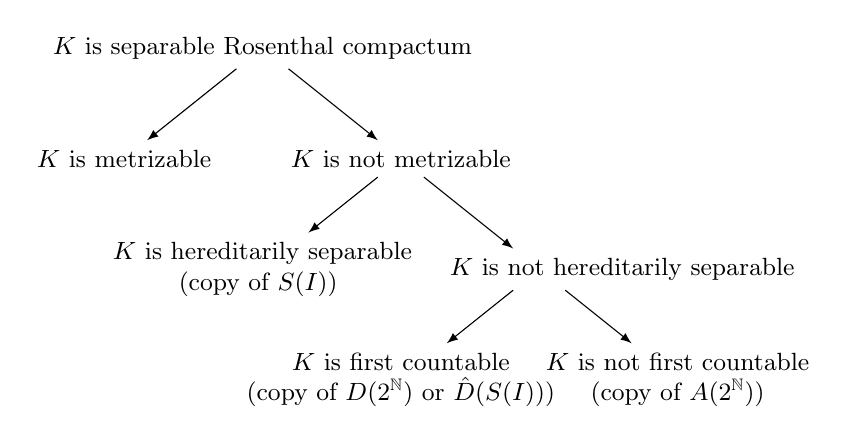
\begin{tikzpicture}[
  grow=down,
  sibling distance=10em,
  level distance=4em,
  edge from parent/.style={draw,-latex},
  every node/.style={font=\small,align=center}
  ]

\node {$K$ is separable Rosenthal compactum}
  child {node {$K$ is metrizable}
  }
  child {node {$K$ is not metrizable}
    child {node {$K$ is hereditarily separable \\ (copy of $S(I)$) \hspace{2cm}}}
    child {node {\hspace{2cm} $K$ is not hereditarily separable}
      child {node {$K$ is first countable \\ (copy of $D(2^\mathbb{N})$ or $\hat{D}(S(I))$)}}
      child {node {$K$ is not first countable \\ (copy of $A(2^\mathbb{N})$)}}
    }
  };

\end{tikzpicture}
\end{center}

Todorčević's Trichotomy suggests that in order to distinguish the classes NIP$_i$, the examples in \ref{E:Rosenthal compacta} are essential.
The following examples show that the levels NIP$_i$ ($i=1,2,3$) may be distinguished by the topological complexity of deep computations.

\begin{exmps}
\label{E: NIP levels}
\hfill
\begin{enumerate}
    \item Let $(L,\mathcal{P},\Gamma)$ be the computation of square root (example \ref{E: computation of square roots} with $\Delta=\Gamma$. 
    We saw that $\overline{\tilde{\Delta}}=\tilde{\Delta}\cup\{\tilde{f}\}\subseteq B_1(\mathcal{L},\mathcal{L})$.
    This corresponds to the Alexandroff compactification of a countable discrete set, which is metrizable. Hence, $\Delta$ is NIP$_3$ but it is not stable, in the sense that $\overline{\tilde{\Delta}}\not\subseteq C(\mathcal{L},\mathcal{L})$.

    \item Let $(L,\mathcal{P},\Gamma)$ be the finite precision threshold classifiers (Section~\ref{subsec:finite_prec_threshold}) with $\Delta=\{\phi_w:w\in 2^{<\mathbb{N}}\}\cup\{\mathbf{0^\infty},\mathbf{1^\infty}\}$.
    We saw that $\overline{\Delta}$ is homeomorphic to the Split Cantor space $S(2^\mathbb{N})$ (Example \ref{E:Rosenthal compacta}(3)), which is hereditarily separable but not metrizable.
    Hence, $\Delta$ is NIP$_2$ but not NIP$_3$.

    \item Let $(L,\mathcal{P},\Gamma)$ be the CCS given by $L=2^{\mathbb{N}}$, $\mathcal{P}=\{P_n:n\in\mathbb{N}\}$ and $\Gamma$ is the semigroup generated by $\Delta=\{\gamma_t:t\in 2^{<\mathbb{N}}\}$, where $P_n:2^\mathbb{N}\rightarrow\{0,1\}$ is the projection map $P_n(x)=x(n)$ and $\gamma_t:L\rightarrow L$ is given by
    \[
	\gamma_t(x)=\begin{cases}
        0^\infty, & \text{if }x<_{\text{lex}}t^\frown0^\infty;\\
        (01)^\infty, & \text{if }t^\frown0^\infty\leq_{\text{lex}} x \leq_{\text{lex}} t^\frown1^\infty;\\
        1^\infty, & \text{if }t^\frown1^\infty<_{\text{lex}}x.
    \end{cases}
    \]
    where $(01)^\infty$ denotes the sequence of alternating bits: $010101\cdots$. 
    As in the other examples, it is not difficult to see that $(L,\mathcal{P},\Gamma)$ satisfies the Extendibility Axiom.
    For example, the condition $t^\frown0^\infty\leq_{\text{lex}} x \leq_{\text{lex}} t^\frown1^\infty$ is equivalent to $x$ extending $t$.
    Observe that the set of deep computations is homeomorphic to $\hat{D}(S(2^{\mathbb{N}}))$ (see Example \ref{E:Rosenthal compacta}(5)).
    This is an example of $\Delta$ which is NIP$_1$ but not NIP$_2$.

    \item Let $(L,\mathcal{P},\Gamma)$ be the finite precision prefix test (Section~\ref{subsec: prefix test}) with $\Delta=\{\psi_w:w\in 2^{<\mathbb{N}}\}$.
    We saw that $\overline{\tilde{\Delta}}$ is homeomorphic to the Extended Alexandroff compactification $\hat{A}(2^\mathbb{N})$ (Example \ref{E:Rosenthal compacta}-(3)), which is separable but not first countable.
    Hence, $\Delta$ is NIP but not NIP$_1$.
\end{enumerate}
\end{exmps}

The definitions provided here for NIP$_i$ ($i=1,2,3$) are topological.
This raises the following question:

\begin{question}
    Is there a non-topological characterization for NIP$_i$, $i=1,2,3$?
\end{question}

\subsection{The Argyros-Dodos-Kanellopoulos heptachotomy, and approximability of deep computation by minimal classes}

In the three separable cases given in \ref{E:Rosenthal compacta}, namely, $\hat{A}(2^\mathbb{N})$, $S(2^\mathbb{N})$ and $\hat{D}(S(2^\mathbb{N}))$, the countable dense subsets are indexed by the binary tree $2^{<\mathbb{N}}$.
This choice of index is useful for two reasons:
\begin{enumerate}
\item
Our emphasis is computational.
Real numbers can be represented as infinite binary sequences, i.e., infinite branches of the binary tree $2^{<\mathbb{N}}$.
We approximate real numbers or binary sequences with elements in $2^{<\mathbb{N}}$, i.e., finite bitstrings.
Indexing standard computations with finite bitstrings allow us to better understand how deep computations arise and how they get approximated.
Computationally, we are interested in the manner (and the efficiency) in which the approximations can occur.
\item
Infinite branches of the binary tree $2^{<\mathbb{N}}$ correspond to the Cantor space $2^{\mathbb{N}}$, the canonical perfect set (in the sense that any Polish space with no isolated points contains a copy of $2^{\mathbb{N}}$).
The use of infinite dimensional Ramsey theory for trees (pioneered by the work of James D. Halpern, Hans Läuchli in \cite{halpern1966partition} and also Keith Milliken in \cite{milliken1981partition}, and Alain Louveau, Saharon Shelah, Boban Velickovic in \cite{louveau_shelah_velickovic_1993}) and perfect sets (Fred Galvin and Andreas Blass in \cite{Blass1981}, Arnold W. Miller in \cite{miller1989infinite}, and Stevo Todorčević in \cite{Todorcevic_1999_CompactSubsetsBaire}) allowed S.A. Argyros, P. Dodos and V. Kanellopoulos in \cite{argyros2008rosenthal} to obtain an improved version of Theorem \ref{T:Todorcevic trichotomy}.
It is no surprise that Ramsey Theory becomes relevant in the study of Rosenthal compacta as it was a key ingredient in Rosenthal's $\ell_1$ Theorem.
For this reason, the main results in \cite{argyros2008rosenthal} (which we cite in this paper) are better explained by indexing Rosenthal compacta with the binary tree.
\end{enumerate}

\begin{defn}
Let $X$ be a Polish space.

\begin{enumerate}
\item
If $I$ is countable and $\{f_i:i\in I\}\subseteq\mathbb{R}^X$, $\{g_i:i\in I\}\subseteq\mathbb{R}^X$ are two pointwise families by $I$, we say that $\{f_i:i\in\ I\}$ and $\{g_i:i\in I\}$ are \emph{equivalent} if and only if the map $f_i\mapsto g_i$ is extended to a homeomorphism from $\overline{\{f_i:i\in I\}}$ to $\overline{\{g_i:i\in I\}}$.
\item
If $\{f_t:t\in 2^{<\mathbb{N}}\}$ is a pointwise bounded family, we say that $\{f_t:t\in 2^{<\mathbb{N}}\}$ is \emph{minimal} if and only if for every dyadic subtree $\{s_t:t\in 2^{<\mathbb{N}}\}$ of $2^{<\mathbb{N}}$, $\{f_{s_t}:t\in 2^{<\mathbb{N}}\}$ is equivalent to $\{f_t:t\in 2^{<\mathbb{N}}\}$.
 \end{enumerate}
\end{defn}

One of the main results in \cite{argyros2008rosenthal} is that, up to equivalence, there are seven minimal families of Rosenthal compacta and that for every relatively compact $\{f_t:t\in 2^{<\mathbb{N}}\}\subseteq B_1(X)$ there is a dyadic subtree $\{s_t:t\in 2^{<\mathbb{N}}\}$ such that $\{f_{s_t}:t\in 2^{<\mathbb{N}}\}$ is equivalent to one of the minimal families.
We shall describe the seven minimal families next.
We follow the same notation as in \cite{argyros2008rosenthal}.
For any node $t\in 2^{<\mathbb{N}}$, let us denote by $t^\frown 0^{\infty}$ ($t^\frown 1^{\infty}$) the infinite binary sequence starting with $t$ and continuing with all $0$'s (respectively, all $1$'s).
Fix a regular dyadic subtree $R=\{s_t:t\in 2^{<\mathbb{N}}\}$ of $2^{<\mathbb{N}}$ (i.e., a dyadic subtree such that every level of $R$ is contained in a level of $2^{<\mathbb{N}}$) with the property that for all $s,s'\in R$, $s^\frown 0^{\infty}\neq s'^\frown 0^\infty$ and $s^\frown 1^{\infty}\neq s'^\frown 1^\infty$.
Given $t\in 2^{<\mathbb{N}}$, let $v_t$ be the characteristic function of the set $\{x\in 2^\mathbb{N}:x \text{ extends } t\}$.
Let $<$ be the lexicographic order in $2^\mathbb{N}$.
Given $a\in 2^{\mathbb{N}}$, let $f^+_a:2^{\mathbb{N}}\rightarrow\{0,1\}$ be the characteristic function of $\{x\in 2^{\mathbb{N}}:a\leq x\}$ and let $f^-_a:2^{\mathbb{N}}\rightarrow\{0,1\}$ be the characteristic function of $\{x\in 2^{\mathbb{N}}:a<x\}$.
Given two maps $f,g:2^{\mathbb{N}}\rightarrow\mathbb{R}$ we denote by $(f,g):2^{\mathbb{N}}\sqcup 2^{\mathbb{N}}\rightarrow\mathbb{R}$ the function which is $f$ on the first copy of $2^{\mathbb{N}}$ and $g$ on the second copy of $2^{\mathbb{N}}$.

\begin{enumerate}
    \item $D_1=\{\frac{1}{|t|+1}v_t:t\in 2^{<\mathbb{N}}\}$.
This is discrete in $\overline{D_1}=A(2^{\mathbb{N}})$.
    \item $D_2=\{s_t^\frown 0^{\infty}:t\in 2^{<\mathbb{N}}\}$.
This is discrete in $\overline{D_2}=2^{\leq N}$.
    \item $D_3=\{f^+_{s_t^\frown 0^\infty}:t\in 2^{<\mathbb{N}}\}$.
This is discrete in $\overline{D_3}=S(2^{\mathbb{N}})$.
    \item $D_4=\{f^-_{s_t^\frown 1^\infty}:t\in 2^{<\mathbb{N}}\}$.
This is discrete in $\overline{D_4}=S(2^{\mathbb{N}})$.
    \item $D_5=\{v_t:t\in 2^{<\mathbb{N}}\}$.
This is discrete in $\overline{D_5}=\hat{A}(2^{\mathbb{N}})$.
    \item $D_6=\{(v_{s_t},s_t^\frown 0^\infty):t\in 2^{<\mathbb{N}}\}$.
This is discrete in $\overline{D_6}=\hat{D}(2^{\mathbb{N}})$.
    \item $D_7=\{(v_{s_t},x^+_{s_t^\frown 0^\infty}):t\in 2^{<\mathbb{N}}\}$.
This is discrete in $\overline{D_7}=\hat{D}(S(2^{\mathbb{N}}))$.
\end{enumerate}

\begin{thm}[Heptachotomy of minimal families, Theorem 2 in \cite{argyros2008rosenthal}]
    Let $X$ be Polish.
For every relatively compact $\{f_{t}:t\in 2^{<\mathbb{N}}\}\subseteq B_1(X)$, there exists $i=1,2,\dots, 7$ and a regular dyadic subtree $\{s_t:t\in 2^{<\mathbb{N}}\}$ of $2^{<\mathbb{N}}$ such that $\{f_{s_t}:t\in 2^{<\mathbb{N}}\}$ is equivalent to $D_i$.
Moreover, all $D_i$ are minimal and mutually non-equivalent.
\end{thm}

The implication of this result for deep computations is the following: 
for any countable set of computations $\Delta$ satisfying the NIP (for some CCS $(L,\mathcal{P},\Gamma)$), we can always find a countable discrete set of deep computations that approximates all the other deep computations.
For example: in the finite precision prefix test example (subsection \ref{subsec: prefix test}), the prefix test computations (family $D_5$) approximate all other deep computations.
However, note that this discrete set $D_i$ may not consist of continuous functions (i.e., they will not be computable in general).
For example, functions in $D_3$ are not continuous.


\section{Randomized versions of NIP and Monte Carlo computability of deep computations}
\label{Measure-theoretic NIP} 

In this section, we replace deterministic computability by probabilistic (`Monte Carlo') computability.
We do not assume that $\mathcal{P}$ is countable.
(The countability assumption on $\mathcal{P}$ played a crucial role in the proof of Theorem \ref{Generalized BFT}, as it makes $\mathbb{R}^\mathcal{P}$ a Polish space.)
The main results of the section are Theorem~\ref{T:NIP and Monte Carlo}  (connecting NIP and Monte Carlo computability) and~\ref{T:Talagrand stability and Monte Carlo}  (connecting Talagrand stability and Monte Carlo computability).

Fundamental in this section is a measure-theoretic version of Theorem \ref{Generalized BFT}, namely,  Theorem~\ref{BFT-2F}. 
For the proof of Theorem \ref{Generalized BFT}, we assumed countability of  $\mathcal{P}$ --- this ensured that $\mathbb{R}^\mathcal{P}$ a Polish space.
In this section, the countability assumption is not needed.

\subsection{NIP and Monte Carlo computability of deep computations}

The \emph{raison d'être} of the Baire class 1 functions is to have a class of functions that are obtained as sequential limit points of continuous functions.
By Fact~\ref{baire}, for perfectly normal $X$, a function $f$ is in $B_1(X,Y)$ if and only if $f^{-1}[U]$ is an $F_\sigma$ subset of $X$ for every open $U\subseteq Y$.
Thus, for such $X$,  functions in $B_1(X,Y)$ are not too far from being continuous.
In this section we will study a more general  class of functions, namely, the class of \emph{universally measurable} functions, which we define next.

\begin{defn}
\label{D:universal measurability}
Given a Hausdorff space $X$ and a measurable space $(Y,\Sigma)$, we say that $f:X\rightarrow Y$ is \emph{universally measurable} (with respect to $\Sigma$) if $f^{-1}(E)$ is $\mu$-measurable for every Radon measure $\mu$ on $X$ and every $E\in\Sigma$.
When $Y=\mathbb{R}$, we will always take $\Sigma=\mathcal{B}(\mathbb{R})$, the Borel $\sigma$-algebra of $\mathbb{R}$.
\end{defn}

If $X$ is a compact (Hausdorff) space, then every Radon measure $\mu$ on $X$ is finite. 
Then, the measure given by $\nu(A):=\mu(A)/\mu(X)$ is a probability measure on $X$ with the same null sets as $\mu$. 
Hence, Radon measures on compact spaces are equivalent to (Radon) probability measures.
We summarize this fact in the next remark:

\begin{rem} 
If $X$ is compact, then a function $f:X\rightarrow\mathbb{R}$ is universally measurable if and only if $f^{-1}(U)$ is $\mu$-measurable for every Radon probability measure $\mu$ on $X$ and every open set $U\subseteq\mathbb{R}$.
\end{rem}

Intuitively, a function is universally measurable if it is ``measurable no matter which reasonable way you try to measure things on its domain".
The concept of universal measurability emerged from work of Kallianpur and Sazonov, in the late 1950's and 1960s --- with later developments by Blackwell, Darst and others ---  building on earlier ideas of Gnedenko and Kolmogorov from the 1950s.
See~\cite[Chapters 1 and 2]{Pap:2002}.

\begin{notn}
Following \cite{BFT_1978_PCompactBaire}, the collection of all universally measurable real-valued functions on $X$ will be denoted by $M_r(X)$.
Given a fixed Radon measure $\mu$ on $X$, the collection of all $\mu$-measurable real-valued functions on $X$ will be denoted by $\mathscr{M}^0(X,\mu)$.
\end{notn}

In the context of deep computations, we are interested in transition maps of a state space $L\subseteq \mathbb{R}^\mathcal{P}$ into itself.
In the product space $\mathbb{R}^\mathcal{P}$, we have two natural $\sigma$-algebras: 
the Borel $\sigma$-algebra, i.e., the $\sigma$-algebra generated by open sets in $\mathbb{R}^\mathcal{P}$, and the cylinder $\sigma$-algebra (i.e., the $\sigma$-algebra generated by the sub-basic open sets in $\mathbb{R}^\mathcal{P}$, that is, the set $\pi_i^{-1}(U)$ with $U\subseteq \mathbb{R}$ open).
In general, the cylinder $\sigma$-algebra is strictly smaller, but when $\mathcal{P}$ is countable, both $\sigma$-algebras coincide.
We will use the cylinder $\sigma$-algebra to define universally measurable maps $f:\mathbb{R}^\mathcal{P}\rightarrow\mathbb{R}^\mathcal{P}$.
The reason for this choice is the following characterization:

\begin{prop}\label{prop:coordinated_univ_meas}
    Let $X$ be a Hausdorff space and $Y=\prod_{i\in I}Y_i$ be any product of measurable spaces $(Y_i,\Sigma_i)$ for $i\in I$.
Let $\Sigma_Y$ be the cylinder $\sigma$-algebra generated by the measurable spaces $(Y_i,\Sigma_i)$.
The following are equivalent for  $f:X\rightarrow Y$.:
    \begin{enumerate}[(i)]
        \item
        $f:X\rightarrow Y$ is universally measurable (with respect to $\Sigma_Y$).
        \item
        $\pi_i\circ f:X\rightarrow Y_i$ is universally measurable (with respect to $\Sigma_i$) for all $i\in I$.
    \end{enumerate}
\end{prop}

\begin{proof}
    (i)$\Rightarrow$(ii) is clear since the projection maps $\pi_i$ are measurable and the composition of measurable functions is measurable.
To prove (ii)$\Rightarrow$(i), suppose that $C=\prod_{i\in I}C_i$ is a measurable cylinder and let $J$ be the finite subset of $I$ such that $C_i\neq Y_i$ for $i\in J$.
Then, $C=\bigcap_{i\in J}\pi_i^{-1}(C_i)$, so $f^{-1}(C)=\bigcap_{i\in J}(\pi_i\circ f)^{-1}(C_i)$ is universally measurable by assumption.
\end{proof}

The preceding proposition says that a transition map is universally measurable if and only if it is universally measurable on all its features; in other words, we can check measurability of a transition just by checking measurability feature by feature.
This is the same as in the Baire class 1 case (compare with Proposition~\ref{prop:Baire-identifications}).

The main result in section \ref{S:Classification} is that, as long as we work with countably many features, PAC-learning (or NIP) corresponds to relative compactness in the space of Baire class 1 functions.
The following result (which does not assume countability of the number of features) gives an analogous characterization of the NIP in terms of universal measurability:

\begin{thm}
[Bourgain-Fremlin-Talagrand, Theorem 2F in \cite{BFT_1978_PCompactBaire}]
\label{BFT-2F}
    Let $X$ be a Hausdorff space and $A\subseteq C(X)$ be pointwise bounded.
The following are equivalent:
    \begin{enumerate}[(i)]
        \item
        $\overline{A}\subseteq M_r(X)$.
        \item 
        For every compact $K\subseteq X$, $A|_K$ satisfies the NIP.
        \item
        For every Radon measure $\mu$ on $X$, $A$ is relatively countably compact in $\mathscr{M}^0(X,\mu)$, i.e., every countable subset of $A$ has a limit point in $\mathscr{M}^0(X,\mu)$.
    \end{enumerate}
\end{thm}

This result allows us to formalize the concept of a deep computation being \emph{Monte Carlo computable}, which we define below (Definition~\ref{D:universally essentially computable}).
To motivate the definition, let us first recall two facts:

\begin{enumerate}
\item
Littlewoood's second principle states that every Lebesgue measurable function is ``nearly continuous''.
The formal statement of this, which is Luzin's theorem, is that if
 $(X,\Sigma ,\mu )$ a Radon measure space and $Y$ is a second-countable topological space (e.g., $Y=\mathbb{R}^\mathcal{P}$ with $\mathcal{P}$ countable) equipped with the Borel $\sigma$-algebra, then any given $f:X\to Y$ is measurable if and only if for every $E\in\Sigma$ and every $\varepsilon>0$ there exists a closed $F\subseteq E$ such that the restriction $f|_F$ is continuous and $\mu(E\backslash F) < \varepsilon$.
\item
Computability of deep computations is characterized in terms of continuous extendibility of computations.
This is at the core of~\cite{alva2024approximability}.
\end{enumerate}

These two facts motivate the following definition:

\begin{defn}
\label{D:universally essentially computable}
    Let $(L,\mathcal{P},\Gamma)$ be a CCS.
We say that a transition $f:L\rightarrow L$ is \emph{universally Monte Carlo computable} if and only if there exists $\tilde f:\mathcal{L}_{\text{sh}}\rightarrow \mathcal{L}_{\text{sh}}$ extending $f$ such that for every sizer $r_\bullet$ there is a sizer $s_\bullet$ such that the restriction $\tilde f|_{\mathcal{L}[r_{\bullet}]}:\mathcal{L}[r_\bullet]\rightarrow\mathcal{L}[s_\bullet]$ is universally measurable, i.e., $\pi_P\circ \tilde f|_{\mathcal{L}[r_{\bullet}]}:\mathcal{L}[r_\bullet]\rightarrow [-s_P,s_P]$ is $\mu$-measurable for every Radon probability measure $\mu$ on $\mathcal{L}[r_\bullet]$ and $P\in\mathcal{P}$.
\end{defn}

\begin{rem}
    Every Radon measure on a compact space (e.g., $\mathcal{L}_{\text{sh}}$) is finite; hence, by proper normalization, it can be treated as a probability measure.
    For this reason, in the context of Monte Carlo computability (\ref{D:universally essentially computable}), we restrict our attention to Radon probability measures instead of  general Radon measures.
\end{rem}


%\subsection{Universal Monte Carlo computability of deep computations}% delete this and move contents before BFT-2F

%\subsection{Bourgain-Fremlin-Talagrand, NIP, and universal Monte Carlo computability of deep computations}
%
%The result in this subsection is a consequence of Theorem~\ref{BFT-2F},
%and it states that PAC-learning (or NIP) implies Monte Carlo computability with respect to any measure.

\begin{thm}
\label{T:NIP and Monte Carlo}
    Let $(L,\mathcal{P},\Gamma)$ be a CCS satisfying the Extendibility Axiom.
Let $R$ be an exhaustive collection of sizers.
Let $\Delta\subseteq\Gamma$ be $R$-confined.
If $\pi_P\circ\Delta|_{L[r_\bullet]}$ satisfies the NIP for all $P\in\mathcal{P}$ and all $r_{\bullet}\in R$, then every deep computation in $\Delta$ is universally Monte Carlo computable.
\end{thm}

\begin{proof}
    Fix $P\in\mathcal{P}$ and $r_\bullet\in R$.
    By the Extendibility Axiom, $\pi_P\circ\tilde\Delta|_{\mathcal{L}[r_\bullet]}$ is a set of pointwise bounded continuous functions on the compact set $\mathcal{L}[r_\bullet]$.
    Since $\pi_P\circ\tilde\Delta|_{L[r_\bullet]}=\pi_P\circ\Delta|_{L[r_\bullet]}$ has the NIP, so does $\pi_P\circ\tilde\Delta|_{\mathcal{L}[r_\bullet]}$ by Lemma \ref{NIP and closure}.
    By Theorem \ref{BFT-2F}, we have $\overline{\pi_P\circ\tilde\Delta|_{\mathcal{L}[r_\bullet]}}\subseteq M_r(\mathcal{L}[r_\bullet])$ for all $r_\bullet\in R$ and $P\in\mathcal{P}$.
    Let $f\in\overline{\Delta}$ be a deep computation.
    Write $f=\mathcal{U}\lim_i\gamma_i$ as an ultralimit of computations in $\Delta$.
    Define $\tilde{f}:=\mathcal{U}\lim_i\tilde{\gamma_i}$.
    Then, $\tilde{f}:\mathcal{L}_{\text{sh}}\rightarrow \mathcal{L}_{\text{sh}}$ extends $f$.
    Since $\Delta$ is $R$-confined we have that $f:L[r_\bullet]\rightarrow L[r_\bullet]$ and $\tilde{f}:\mathcal{L}[r_\bullet]\rightarrow \mathcal{L}[r_\bullet]$ for all $r_\bullet\in R$.
    Lastly, note that for all $r_\bullet\in R$ and $P\in\mathcal{P}$ we have that $\pi_P \circ \tilde{f}|_{\mathcal{L}[r_\bullet]}\in \overline{\pi_P\circ\tilde\Delta|_{\mathcal{L}[r_\bullet]}}\subseteq M_r(\mathcal{L}[r_\bullet])$.
\end{proof}

\begin{question}
Under the same assumptions of the preceding theorem, suppose that every deep computation of $\Delta$ is universally Monte Carlo computable.
Must $\pi_P\circ\Delta|_{L[r_\bullet]}$ have the NIP for all $P\in\mathcal{P}$ and all $r_{\bullet}\in R$?
\end{question}

\subsection{Talagrand stability and Monte Carlo computability of deep computations}

There is another notion closely related to NIP, introduced by Talagrand in \cite{talagrand1984pettis} while studying Pettis integration.
Suppose that $X$ is a compact Hausdorff space and $A\subseteq \mathbb{R}^X$.
Let $\mu$ be a Radon probability measure on $X$.
Given a $\mu$-measurable set $E\subseteq X$, a positive integer $k$ and real numbers $a<b$, we write:

\[
	D_k(A,E,a,b)=\bigcup_{f\in A}\{x\in E^{2k}:f(x_{2i})\leq a, \hspace{1mm} f(x_{2i+1})\geq b \hspace{1mm}{\text{ for all }i<k} \}.
\]

We say that $A$ is \emph{Talagrand $\mu$-stable} if and only if for every $\mu$-measurable set $E\subseteq X$ of positive measure and for every $a<b$ there is a $k\geq 1$ such that
\[
(\mu^{2k})^*(D_k(A,E,a,b))<(\mu(E))^{2k},
\]
where $\mu^*$ denotes the outer measure (we need to work with outer measure since the sets $D_k(A,E,a,b)$ need not be $\mu^{2k}$-measurable).
The inequality certainly holds when $A$ is a countable set of continuous (or $\mu$-measurable) functions.

The main result of this section is that deep computations, i.e., limit points of a Talagrand stable set of computations are Monte Carlo computable; this is Theorem~\ref{T:Talagrand stability and Monte Carlo} below.
We now prove that limit points of a Talagrand $\mu$-stable set are $\mu$-measurable.
But first,  let us state  the following useful characterization of measurable functions (compare with Fact \ref{baire}):

\begin{fact}[Lemma 413G in \cite{fremlin2003vol4}]\label{fact: measurable functions characterization}
    Suppose that $(X,\Sigma,\mu)$ is a measure space and $\mathcal{K}\subseteq\Sigma$ is a collection of measurable sets satisfying the following conditions:
    \begin{enumerate}
        \item $(X,\Sigma,\mu)$ is complete, i.e., for all $E\in\Sigma$ with $\mu(E)=0$ and $F\subseteq E$ we have $F\in\Sigma$.
        \item $(X,\Sigma,\mu)$ is semi-finite, i.e., for all $E\in\Sigma$ with $\mu(E)=\infty$ there exists $F\subseteq E$ such that $F\in\Sigma$ and $0<\mu(F)<\infty$.
        \item $(X,\Sigma,\mu)$ is saturated, i.e., $E\in\Sigma$ if and only if $E\cap F\in\Sigma$ for all $F\in\Sigma$ with $\mu(F)<\infty$.
        \item $(X,\Sigma,\mu)$ is inner regular with respect to $\mathcal{K}$, i.e., for all $E\in\Sigma$
        \[
	\mu(E)=\sup\{\mu(K):K\in\mathcal{K} \text{ and } K\subseteq E\}.
        \]
    \end{enumerate}
    (In particular, if $X$ is compact Hausdorff, $\mu$ is a Radon probability measure on $X$, $\Sigma$ is the completion of the Borel $\sigma$-algebra by $\mu$, and $\mathcal{K}$ is the collection of compact subsets of $X$, all these conditions hold).
    Then, $f:X\rightarrow\mathbb{R}$ is measurable if and only if for every $K\in\mathcal{K}$ with $0<\mu(K)<\infty$ and $a<b$, either $\mu^*(P)<\mu(K)$ or $\mu^*(Q)<\mu(K)$ where $P=\{x\in K:f(x)\leq a\}$ and $Q=\{x\in K:f(x)\geq b\}$.
\end{fact}

The following technical lemma will be instrumental for proving Proposition~\ref{prop:Talagrand implies NIP}, which, in turn, will yield the main result of the subsection, namely Theorem~\ref{T:Talagrand stability and Monte Carlo}.

\begin{lem}\label{talagrand stable is relatively compact}
    If $A$ is Talagrand $\mu$-stable, then $\overline{A}$ is also Talagrand $\mu$-stable and $\overline{A}\subseteq\mathscr{M}^0(X,\mu)$.
\end{lem}

\begin{proof}
    First, we claim that a subset of a $\mu$-stable set is $\mu$-stable.
    To see this, suppose that $A\subseteq B$ and $B$ is $\mu$-stable.
    Fix any $\mu$-measurable $E\subseteq X$ of positive measure and $a<b$.
    Let $k\geq 1$ such that
    \[
    (\mu^{2k})^*(D_k(B,E,a,b))<(\mu(E))^{2k}.
    \]
    Since $A\subseteq B$, we have $D_k(A,E,a,b)\subseteq D_k(B,E,a,b)$; therefore,
    \[
    (\mu^{2k})^*(D_k(A,E,a,b))\leq (\mu^{2k})^*(D_k(B,E,a,b))<(\mu(E))^{2k}.
    \]
    We now show that $\overline{A}$ is $\mu$-stable.
    Fix $E\subseteq X$ measurable with positive measure and $a<b$.
    Let $a'<b'$ be such that $a<a'<b'<b$.
    Since $A$ is $\mu$-stable, let $k\geq 1$ be such that
    \[
    (\mu^{2k})^*(D_k(A,E,a',b'))<(\mu(E))^{2k}.
    \]
    If $x\in D_k(\overline{A},E,a,b)$, then there is $f\in\overline{A}$ such that $f(x_{2i})\leq a<a'$ and $f(x_{2i+1})\geq b>b'$ for all $i<k$.
    By definition of pointwise convergence topology, there exists $g\in A$ such that $g(x_{2i})<a'$ and $g(x_{2i+1})>b'$ for all $i<k$.
    Hence, $x\in D_k(A,E,a',b')$.
    We have shown that $D_k(\overline{A},E,a,b)\subseteq D_k(A,E,a',b')$; hence,
    \[
    (\mu^{2k})^*(D_k(\overline{A},E,a,b))\leq (\mu^{2k})^*(D_k(A,E,a',b'))<(\mu(E))^{2k}.
    \]
    It suffices to show that $\overline{A}\subseteq \mathscr{M}^0(X,\mu)$.
    Suppose that there exists $f\in\overline{A}$ such that $f\notin \mathscr{M}^0(X,\mu)$.
    By fact \ref{fact: measurable functions characterization}, there exists a $\mu$-measurable set $E$ of positive measure and $a<b$ such that $\mu^*(P)=\mu^*(Q)=\mu(E)$ where $P=\{x\in E: f(x)\leq a\}$ and $Q=\{x\in E: f(x)\geq b\}$.
    Then, for any $k\geq 1$: $(P\times Q)^k\subseteq D_k(\{f\},E,a,b)$, so $(\mu^{2k})^*(D_k(\{f\},E,a,b))=(\mu^*(P)\mu^*(Q))^k=(\mu(E))^{2k}$.
    Thus, $\{f\}$ is not $\mu$-stable. However,  we argued above that a subset of a $\mu$-stable set must be $\mu$-stable,
    so we have a contradiction.
\end{proof}

\begin{defn}
We say that $A$ is \emph{universally Talagrand stable} if $A$ is Talagrand $\mu$-stable for every Radon probability measure $\mu$ on $X$.
\end{defn}

We first observe that universal Talagrand stability corresponds to a complexity class smaller than or equal to the NIP class:

\begin{prop}\label{prop:Talagrand implies NIP}
    Let $X$ be a compact Hausdorff space and $A\subseteq C(X)$ be pointwise bounded.
If $A$ is universally Talagrand stable, then $A$ satisfies the NIP.
\end{prop}

\begin{proof}
    By Theorem \ref{BFT-2F}, it suffices to show that $A$ is relatively countably compact in $\mathscr{M}^0(X,\mu)$ for every Radon probability measure $\mu$ on $X$.
Since $A$ is Talagrand $\mu$-stable for any such $\mu$, we have $\overline{A}\subseteq\mathscr{M}^0(X,\mu)$ by Lemma \ref{talagrand stable is relatively compact}.
In particular, $A$ is relatively countably compact in $\mathscr{M}^0(X,\mu)$.
\end{proof}

\begin{cor}
\label{T:Talagrand stability and Monte Carlo}
    Let $(L,\mathcal{P},\Gamma)$ be a CCS satisfying the Extendibility Axiom.
If $\pi_P\circ\Delta|_{L[r_\bullet]}$ is universally Talagrand stable for all $P\in\mathcal{P}$ and all sizers $r_{\bullet}$, then every deep computation is universally Monte Carlo computable.
\end{cor}

\begin{proof}
    This is a direct consequence of Proposition \ref{prop:Talagrand implies NIP} and Theorem~\ref{T:NIP and Monte Carlo}.
\end{proof}

In the context of deep computations, we have identified two ways to obtain Monte Carlo computability, namely,
NIP/PAC and Talagrand stability. 
It is natural to ask whether these two notions are equivalent. 
The following results show that, even in the simple case of countably many computations, this question is sensitive to the set-theoretic axioms. 
On the one hand, it is consistent (with respect to the standard ZFC axioms of set theory) that these two classes are the same:

\begin{thm}[Talagrand, Theorem 9-3-1(a) in \cite{talagrand1984pettis}]
\label{T:nip implies talagrand stability}
    Let $X$ be a compact Hausdorff space and $A\subseteq M_r(X)$ be countable and pointwise bounded.
Assume that $[0,1]$ is not the union of $<\mathfrak{c}$ closed measure zero sets.
If $A$ satisfies the NIP, then $A$ is universally Talagrand stable.
\end{thm}

(The assumption that $[0,1]$ is not the union of $<\mathfrak{c}$ closed measure zero sets is a consequence of, for example, the Continuum Hypothesis.)

On the other hand, by fixing a particular well-known measure, namely the Lebesgue measure, we see that the other case is also consistent:

\begin{thm}[Fremlin, Shelah, \cite{fremlin1993pointwise}]
    It is consistent with the usual axioms of set theory that there exists a countable pointwise bounded set of Lebesgue measurable functions with the NIP which is not Talagrand stable with respect to Lebesgue measure.
\end{thm}

Notice that the preceding two results apply to sets of measurable functions, a class of functions larger than the class of continuous functions.
However, by the Extendibility Axiom, finitary computations are continuous, i.e., if $A$ is a set of computations, then $A\subseteq C_p(X)$.



\section{Conclusion}

We have seen how the tools of model theory and the topology of function spaces can give us new insights into classifying the difficulty of computations.
In future papers, we plan to extend this research in a variety of directions. 
A direction of particular interest to us  is replacing classical computation by quantum computation.
Topologically, our results so far are not optimal because of their restriction to Polish spaces. 
We expect to extend most of them to $K$-countably determined (Lindelöf $\Sigma$) spaces or  $K$-analytic spaces, which have previously been used in functional analysis --- see e.g., Kakol \emph{et al}~\cite{Kakol-Kubis-Lopez-Pelicer-Sobota:2025}.
Our restricting our considerations to continuous and Baire class~1 functions can be relaxed by applying more high-powered model-theoretic and topological techniques. 
This is work in progress. 
We have hinted at applications to deep equilibria; see~\cite{alva2024approximability}.
In another direction, we have hinted at the role additional set-theoretic axioms may play. 
Since real world computations are finite and hence do not depend on other than the usual set-theoretic axioms, in principle we can assume these axioms and then dispense with them;
however, this is delicate, since many of our techniques involve infinite sets so we have to check that our assertions are sufficiently simple so as to be \emph{absolute}, i.e., unaffected by additional axioms. 
We hope that this paper, the preceding one~\cite{alva2024approximability}, and the future ones will stimulate interactions among these three seemingly unrelated fields of research.




%%%%%%%%%%%%%%%%%%%%%%%%%%%%%%%%%%%%%%%%%%%%%%%%%%%%%%%%%%%%%%%%%%%%%%%%%%



%%%%%%%%%%%%%%%%%%%%%%%%%%%%%%%%%%%%%%%%%%%%%%%%%%%%%%%%%%%%%%%%%

%\begin{thebibliography}{9}



\bibliographystyle{alpha}
%\nocite{*}
\bibliography{bib}

%\end{thebibliography}
\end{document}
